\begin{refsection}
\chapter{Mutations Involving Glutamic Acid Sidechains Modulate Na$^+$ Conduction}

Contributions by Christopher Ing (CI), Nilu Chakrabarti (NC), Regis Pomes (RP), and William A. Catterall (WC): C.I., N.C, and R.P. designed the research. Simulations were performed by N.C. and C.I. Data analysis was performed by C.I. and R.P. The manuscript was written by C.I., and R.P. 

\newpage

\section{Summary}

	Dynamic fluctuations of channel ligands are integral to ion permeation and selectivity in cation channels. Microsecond-timescale molecular dynamics simulations of the bacterial voltage-gated Nav channel reveal that glutamic acid side chains within the SF can adopt both a down-facing and up-facing state, and that these conformational fluctuations can catalyze Na$^+$ conduction and result in Na$^+$ selectivity over K$^+$. This process may involve variable numbers of Glu sidechains and result in coordination to a variable number of partially hydrated cations. These channel fluctuations can dynamically modulate the effective diameter and charge of the SF in response to permeating ions, and are found to catalyze the conduction of Na$^+$ by providing a diffusive free energy landscape. These fluctuations enable selective permeation of Na$^+$ by supporting multi-ion occupancy within the SF while simultaneously restricting K$^+$ movement due to geometric constraints. The role of channel fluctuations is evident from simulations where glutamic acid sidechains are conformationally restricted to an up-facing state, which does not facilitate rapid transport of Na$^+$ in agreement with experimental conductance rates. However, this molecular mechanism has not been verified experimentally.
	
	We propose mutations to the hydrogen bonding environment around these carboxylate side chains, that modulate conformational isomerization and alter ion conduction properties of Na$^+$ and K$^+$. Mutations which remove protein-protein interactions involving carboxylate sidechains to neighbouring hydroxyl sidechains of serine sidechains (S178A, S180A, S178A/S180A) are found to increase the propensity for glutamic acid side chains to adopt a down-facing state and alter ionic binding within the SF. Conversely, mutations which increase the likelihood that carboxylate sidechains will form protein-protein interactions with neighbouring serine hydroxyl groups (Y168F) are found to increase the propensity to adopt a up-facing state, and ionic conduction is found to be impeded. The Y168F mutation results in a Na$^+$ and K$^+$ conduction mechanism that is consistent with simulations conducted with conformationally restricted glutamic acid sidechains. In all systems, we examine the free energy of ion conduction for both Na$^+$ and K$^+$ and make predictions about expected perturbations to experimental observables such as ionic conduction rates and selectivity ratios. Together, this work demonstrates that the degree of conformational isomerization of glutamic acid side chains can modulate ionic conduction and selectivity, and that this prediction may be experimentally tested using site-directed mutagenesis and electrophysiology.
	
\section{Introduction}

%Voltage-gated sodium channels initiate action potentials in excitable cells through selective transport of Na$^+$ across biological membranes \cite{Hille:2001tw}. Selectivity for Na$^+$ over other biological cations like K$^+$ and Ca2+ is controlled by a narrow constriction within the ion conduction pathway referred to as the selectivity filter. 

The bacterial voltage-gated sodium channel selectivity filter is homo-tetrameric and is lined with backbone carbonyl groups, carboxylate side chains, and serine hydroxyl groups \cite{Payandeh:2012ib}. Carboxylate side chains have been identified near or within the SF of several other ion channels from disparate protein families \cite{Li:2017ex,Paulsen:2015bp,Grieben:2016ij}, but their role in ionic conduction is not well understood.  In K$^+$ channels, SF channels have been linked to ion conduction \cite{Kratochvil:2016jx,Noskov:2004tv}, and structures solved of the KcsA channel in low [K$^+$] demonstrate that the SF is also capable of collapse as a mechanism for inactivation \cite{Zhou:2001vo}. What is the extent to which SF fluctuations play a role in Na$^+$ conduction in Na$^+$ channels?

In the bacterial voltage-gated sodium channel, our previous data support the hypothesis that sidechain conformational isomerization, or dunking, plays a critical role in selective Na$^+$ conduction \cite{Chakrabarti:2013kd}. Our molecular simulations demonstrate that glutamic acid side chains are essential ligands of Na$^+$ and that their conformational isomerization is coupled to binding and movement of Na$^+$ \cite{Chakrabarti:2013kd}. Selective permeation of Na$^+$ through the SF occurs through a loosely-coupled knock-on mechanism involving 2-3 partially hydrated Na$^+$ which directly coordinate 1-4 glutamic acid sidechains. Furthermore, we've determined that by artificially preventing glutamic acid fluctuations we observe a major destabilization of Na$^+$ binding within the SF (Chapter 5). Multiple studies have since analyzed the role of glutamic acid sidechain fluctuations in Na$^+$ conduction \cite{Ke:2014fy,Boiteux:2014ut,Domene:2015kj,Furini:2014gv}. A similar mechanism has been described for the glutamate ring of the cation-selective nicotinic acetylcholine receptor \cite{Harpole:2014gu}. Our simulations also support the link between ionic selectivity and channel fluctuations. In studies of Na$^+$ and K$^+$ binding within the bacterial voltage-gated sodium channel, multi-ion occupancy of the SF results in a diffusive energy landscape for Na$^+$ but not for K$^+$. Due to geometric constraints of E177 sidechains within the SF and a difference in ionic radii, a free-energy barrier prevents rapid diffusion of K$^+$ in favour of Na$^+$. Together, these factors strengthen the connection between channel fluctuations and selective ionic conduction, but experimental evidence supporting this hypothesis has so far been scarce.

Crystallographic structures do not identify increased temperature factors for atoms within the SF. In both open and closed structures of voltage-gated sodium channels, there are only sub-angstrom variations in backbone and sidechain root-mean square deviation of the SF \cite{Sula:2017jx,Sula:2017hu,Lenaeus:2017cy} with the exception of a putative inactivated state of the NavAb channel with an asymmetrically closed SF \cite{Payandeh:2013ex}. Electron density assigned to Na$^+$ within the SF of a high-resolution crystal structure of NavMs does not indicate that glutamic acid sidechains adopt alternative conformations to coordinate bound ions \cite{Naylor:2016cu}. In the structure of the eukaryotic channel NavPas, the orientation of Asp and Glu side chains could not be assigned in the SF due to radiation damage \cite{Shen:2017df}. Nonetheless, this lack of structural evidence for channel fluctuations does not preclude dynamics of side chains under physiological conditions. On the basis of molecular dynamics simulations, can we propose channel mutations that may be used to measure the effect of E177 fluctuations on ionic conduction?

In the experiments presented here, we extend our previous studies of Na$^+$ and K$^+$ permeation in NaVAb \cite{Chakrabarti:2013kd} with simulations of novel channel mutants that modulate Na$^+$ conduction. Specifically, we perform multiple all-atom 1000-ns molecular dynamics repeats, and compare Na$^+$ binding and permeation properties of the WT channel and four mutants, S178A, S180A, S178/S180A, and Y168F. The former three mutants increase conformational isomerization and the latter mutant decreases conformational isomerization. A strong relationship is found between this propensity for E177 conformational isomerization and the binding of Na$^+$ within the SF. When drawing comparison between Na$^+$ and K$^+$, we expect that these mutants, particularly those preventing dunking, will perturb or eliminate selectivity for Na$^+$. These results provide the foundation for experimental validation of glutamic acid side chain fluctuations as a determining factor for the mechanism of conduction and selectivity in Nav channels.

\section{Results}

Channel fluctuations involving glutamic acid side chains occur spontaneously in brute-force molecular dynamics studies of the sodium channel NavAb. We have shown how binding to permeating cations displaces the conformational equilibrium towards the down-facing or dunked state of the Glu side chains \cite{Chakrabarti:2013kd}. To further characterize the factors controlling the conformational equilibrium, we analyze the protein-protein interactions involving E177. In a representative molecular rendering from simulations, we observe multiple hydrogen bonding partners for glutamic acid side chain E177 of the NavAb SF in the up-facing conformation, whereas no protein-protein hydrogen bonds were observed in the dunked state (Fig. \ref{fig:nav6fig1}) (unless one or more E177 were protonated, in which case it could form hydrogen bonds with unprotonated glutamic acid sidechains). A single E177 carboxylate group can interact with one or more serine hydroxyl groups of S178 or S180. One of these primary ligands of E177, S180, was found to interact with a neighboring Y168F side chain, preventing the hydroxyl side chain from acting hydrogen bond donor (Fig. \ref{fig:nav6fig1} A-B). Hydrogen bonds may be formed individually between E177 and S178 of the same subunit, E177 and S180 of the adjacent subunit, or both simultaneously (Fig. \ref{fig:nav6fig1} A-D). In the absence of these interactions, E177 may adopt a lumen-facing state, directly coordinating permeating Na$^+$ within the SF (Fig. \ref{fig:nav6fig1} E). In the presence of these interactions, E177 adopts an outfacing state, near the crystallographic orientation (Fig. \ref{fig:nav6fig1} F-G). 

\begin{figure}[!ptb]
\centering
\includegraphics[width=0.8\textwidth]{nav6/Nav6Fig1}
\caption[Molecular rendering of the hydrogen bonding network surrounding E177 in Na\textsubscript{V}Ab]{\textbf{Molecular rendering of the hydrogen bonding network surrounding E177 in Na\textsubscript{V}Ab}. (\textbf{A}) Structure of the NavAb selectivity filter from molecular simulation from the extracellular view, with selectivity filter residues E177, S178, and surrounding residues S180 and Y168 shown. (A-B) The crystallographic conformation of E177, hydrogen bonded to S178, along with the adjacent S180 hydrogen bonded to Y168. (C) Alternate conformation of E177, hydrogen bonded to S180, which is no longer interacting with Y168. (D) Alternate conformation of E177, hydrogen bonded to both S178 and S180. (E-H) Structure of the NavAb selectivity filter from a side-view orientation, showing (E) conformational isomerization of a single E177 side chain to coordinate ions, and (F-H) the three E177 hydrogen bonding partners shown in (A-D).}
\label{fig:nav6fig1}
\end{figure}

	Na$^+$ movement through the SF is coupled to the conformational isomerization of the side chains of E177 between an `undunked' and `dunked' state which may occur on a timescale of tens of nanoseconds \cite{Chakrabarti:2013kd}.  Specifically, cation binding shifts the conformational equilibrium of E177 from the crystallographically-observed conformer, ($\chi_1$,$\chi_2$) = (t, g$^+$), to the conformer where the carboxylate group points into the channel lumen, ($\chi_1$,$\chi_2$) = (t, g$^-$). We computed the percentage of frames where E177 adopted a dunked conformation in the presence of Na$^+$ or K$^+$ (Fig. \ref{fig:nav6fig2}). In WT simulations of Na$^+$, E177 side chains adopt a dunked conformation in 45$\pm$5\% of frames, which provides a reference value to compare our mutant channels. In the S178A and S180A mutants, E177 dunking is promoted to 83$\pm$4\% and 76$\pm$4\% of frames, respectively. By introducing both Ser to Ala mutations in the S178A/S180A mutant, E177 dunking increased to 87$\pm$3\% of frames. Conversely, the Y168F mutation promoted the interaction of E177 to S180, resulting in an overall reduction of E177 dunking to 6$\pm$2\% of frames. The percentage of dunked conformations were within error for Na$^+$ and K$^+$ for all models with the exception of S180A, which promoted dunking to 62$\pm$2\% for K$^+$. 

\begin{figure}[!ptb]
\centering
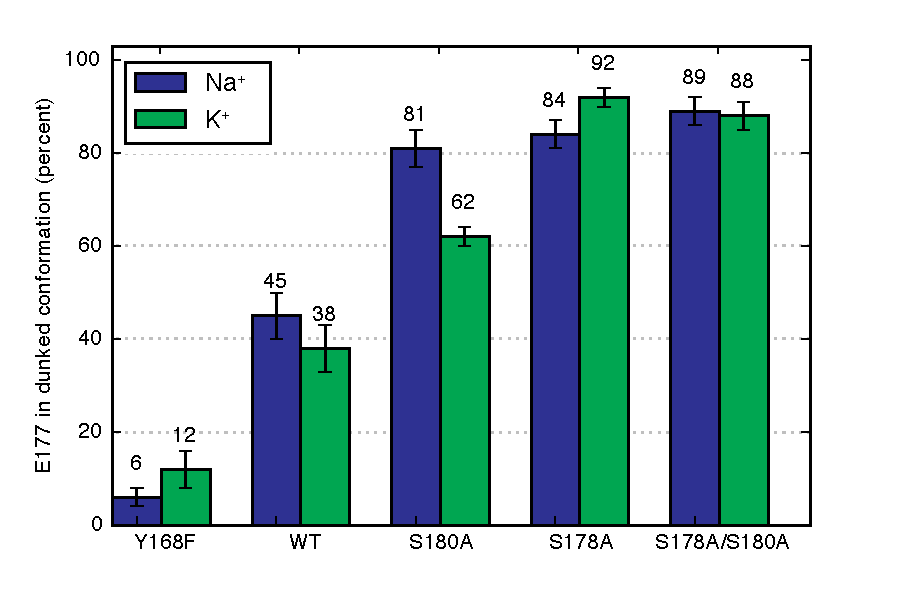
\includegraphics[width=0.5\textwidth]{nav6/Nav6Fig2}
\caption[E177 side chain conformational isomerization]{\textbf{E177 side chain conformational isomerization}. (\textbf{A}) The mean percentage of simulation time in the E177 side chain adopted a lumen-facing state. Data is shown for Y168F, WT, S180A, S178A, and S178A/S180A in the presence of either Na$^+$ (blue) or K$^+$ (green). Error bars are computed as the standard error of mean across all simulation repeats.}
\label{fig:nav6fig2}
\end{figure}

Conformational isomerization alters the free energy of ion conduction within the SF. We report the one-dimensional potential of mean force for Na$^+$ (Fig. \ref{fig:nav6fig3} A,C) and K$^+$ (Fig. \ref{fig:nav6fig3} B,D) movement along the pore axis for the WT model and all mutants studied. Although ionic conduction in Nav channels is a multi-ion process, by projecting the multi-dimensional free energy of ionic conduction onto the channel axis, we capture the essential differences in the multi-ion conduction process. The 1D PMF for Na$^+$ and K$^+$ in the WT model (Fig. \ref{fig:nav6fig3} A-B, black line) highlight the `E', `EL', and `LT' binding sites of the SF, broadly located at positions -4, 0, and 4 \AA, respectively. Differences in the 1D free energy profile for Na$^+$ and K$^+$ in the WT datasets result from a difference in the multi-ion conduction mechanism. A relatively minor difference exists between the free energy of ion conduction in the WT and S180A models (Fig. \ref{fig:nav6fig3} A-B), suggesting that while glutamic acid fluctuations have nearly doubled, ion binding is largely unperturbed and the diffusive energy landscape of the SF is preserved. In the S180A mutant, increased dunking resulted in an increase of SF occupancy by Na$^+$ from 2.1$\pm$0.1 to 2.6$\pm$0.1 ions compared to the WT model, stemming primarily from greater `EL' binding (\Cref{fig:nav6figS2,fig:nav6figS3}). In the S178A and S178A/S180A mutants, increased E177 dunking reduces binding at the `high-field strength' site (referred to as the `E' site in our work), which has the largest effect on K$^+$ binding. Although dunking was increased in the S178A and S178A/S180A models, the commensurate decrease of `E' binding resulted in no net change of SF occupancy by Na$^+$, again due to increased `EL' binding (\Cref{fig:nav6figS4,fig:nav6figS5}). In all three Ser-to-Ala mutants, increased E177 dunking reduces a small barrier within the SF between the `EL' and `LT' sites. The free energy of ion conduction in the Y168F mutant (Fig. \ref{fig:nav6fig3} C-D), having greatly reduced E177 conformational isomerization, results in a significant barrier between the `E' and `LT' states that permits rapid Na$^+$ diffusion, and to a lesser extent the conduction of K$^+$. We examined the 1D PMF for ion conduction in the limit of 0\% E177 dunking for the WT model, referred to as `E177 DR', and barrier for ion conduction was within error of the Y168F mutant. In both reduced dunking models, SF occupancy of Na$^+$ was decreased to 1.99$\pm$0.01 and 1.95$\pm$0.02 ions in Y168F and E177 DR, respectively, compared to 2.1$\pm$0.1 in the WT (Fig. \ref{fig:nav6figS6}). This suggests that the crystallographic state of the E177 in the SF can be effectively stabilized by the Y168F mutation. 

\begin{figure}[!ptb]
\centering
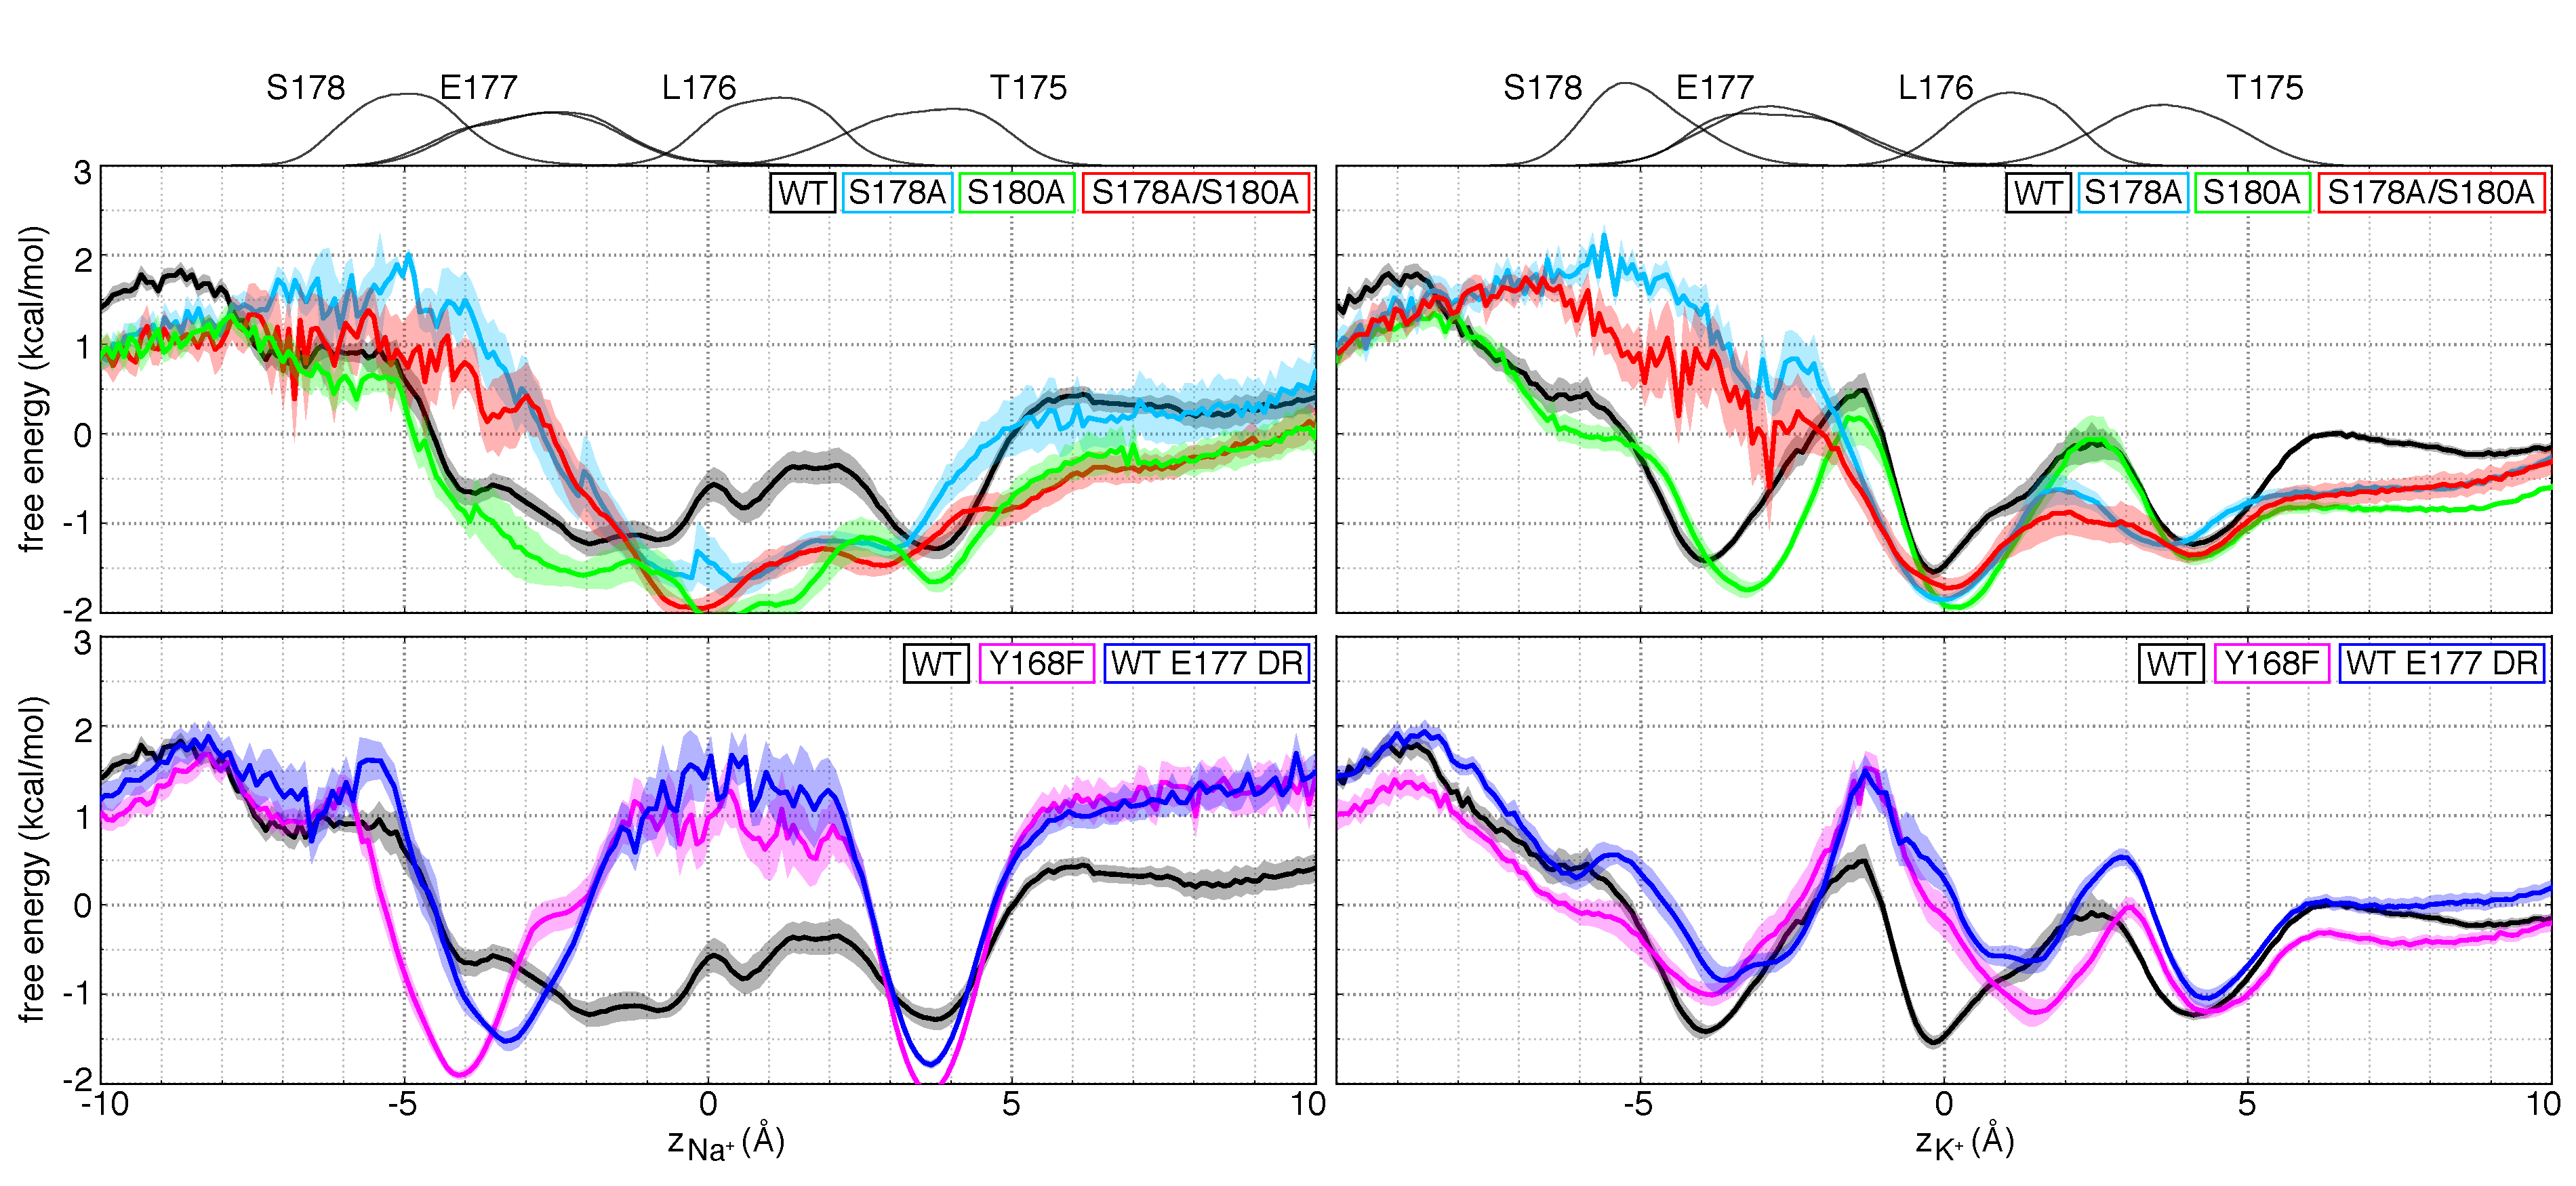
\includegraphics[width=0.9\textwidth]{nav6/Nav6Fig3}
\caption[Potential of mean-force (PMF) for the movement of Na$^+$ and K$^+$ along the channel axis]{\textbf{Potential of mean-force (PMF) for the movement of Na$^+$ and K$^+$ along the channel axis}. (\textbf{A}) One-dimensional multi-ion PMFs for pure Na$^+$ (left column) or K$^+$ (right column) movement along the channel axis in the (A-B) WT, S178A, S180A, S178A/S180A models. One-dimensional PMFs are also shown for the (C-D) WT, Y168F, and WT model with E177 dihedral restraints (E177 DR). The reference state (zero free energy) is defined as the bulk extracellular value for Na$^+$ or K$^+$ in each dataset separately. The axial distribution of pore-lining oxygen atoms of S178, E177, L176, and T175 are shown from WT simulations above both Na$^+$ and K$^+$ plots.}
\label{fig:nav6fig3}
\end{figure}

In an alternate forcefield with higher channel occupancy ($\sim 2.6$ using OPLS compared to $\sim 2.2$ using CHARMM), simulations of S178A, S180A, S178A/S180A, and Y168F were recomputed. A linear relationship between the aforementioned mutations and the degree of conformational isomerization of E177 was observed for simulations with Na$^+$ (Fig. \ref{fig:nav6figS1} A), although the perturbation induced by the Y168F mutation was far less dramatic (44$\pm$3\% in OPLS compared to 6$\pm$2\% in CHARMM). Simulations of these mutants performed in the absence of bulk ions reveal that native channel fluctuations may be perturbed, even though low ion conditions are unlikely to occur in the physiological state of the channel. For example, in the absence of salt, Glu adopted a dunked conformation in 5$\pm$2 frames for WT, compared to 33$\pm$2 frames for S178A. However, these mutations did not directly translate into differences in the 1D PMF for Na$^+$ (Fig. \ref{fig:nav6figS1} B), suggesting that our mechanisms may be sensitive to force field parameterization. Additional experimental validation must be performed in order to confirm the effect of conformational isomerization of Glu sidechains on ionic conductance.

\begin{figure}[!ptb]
\centering
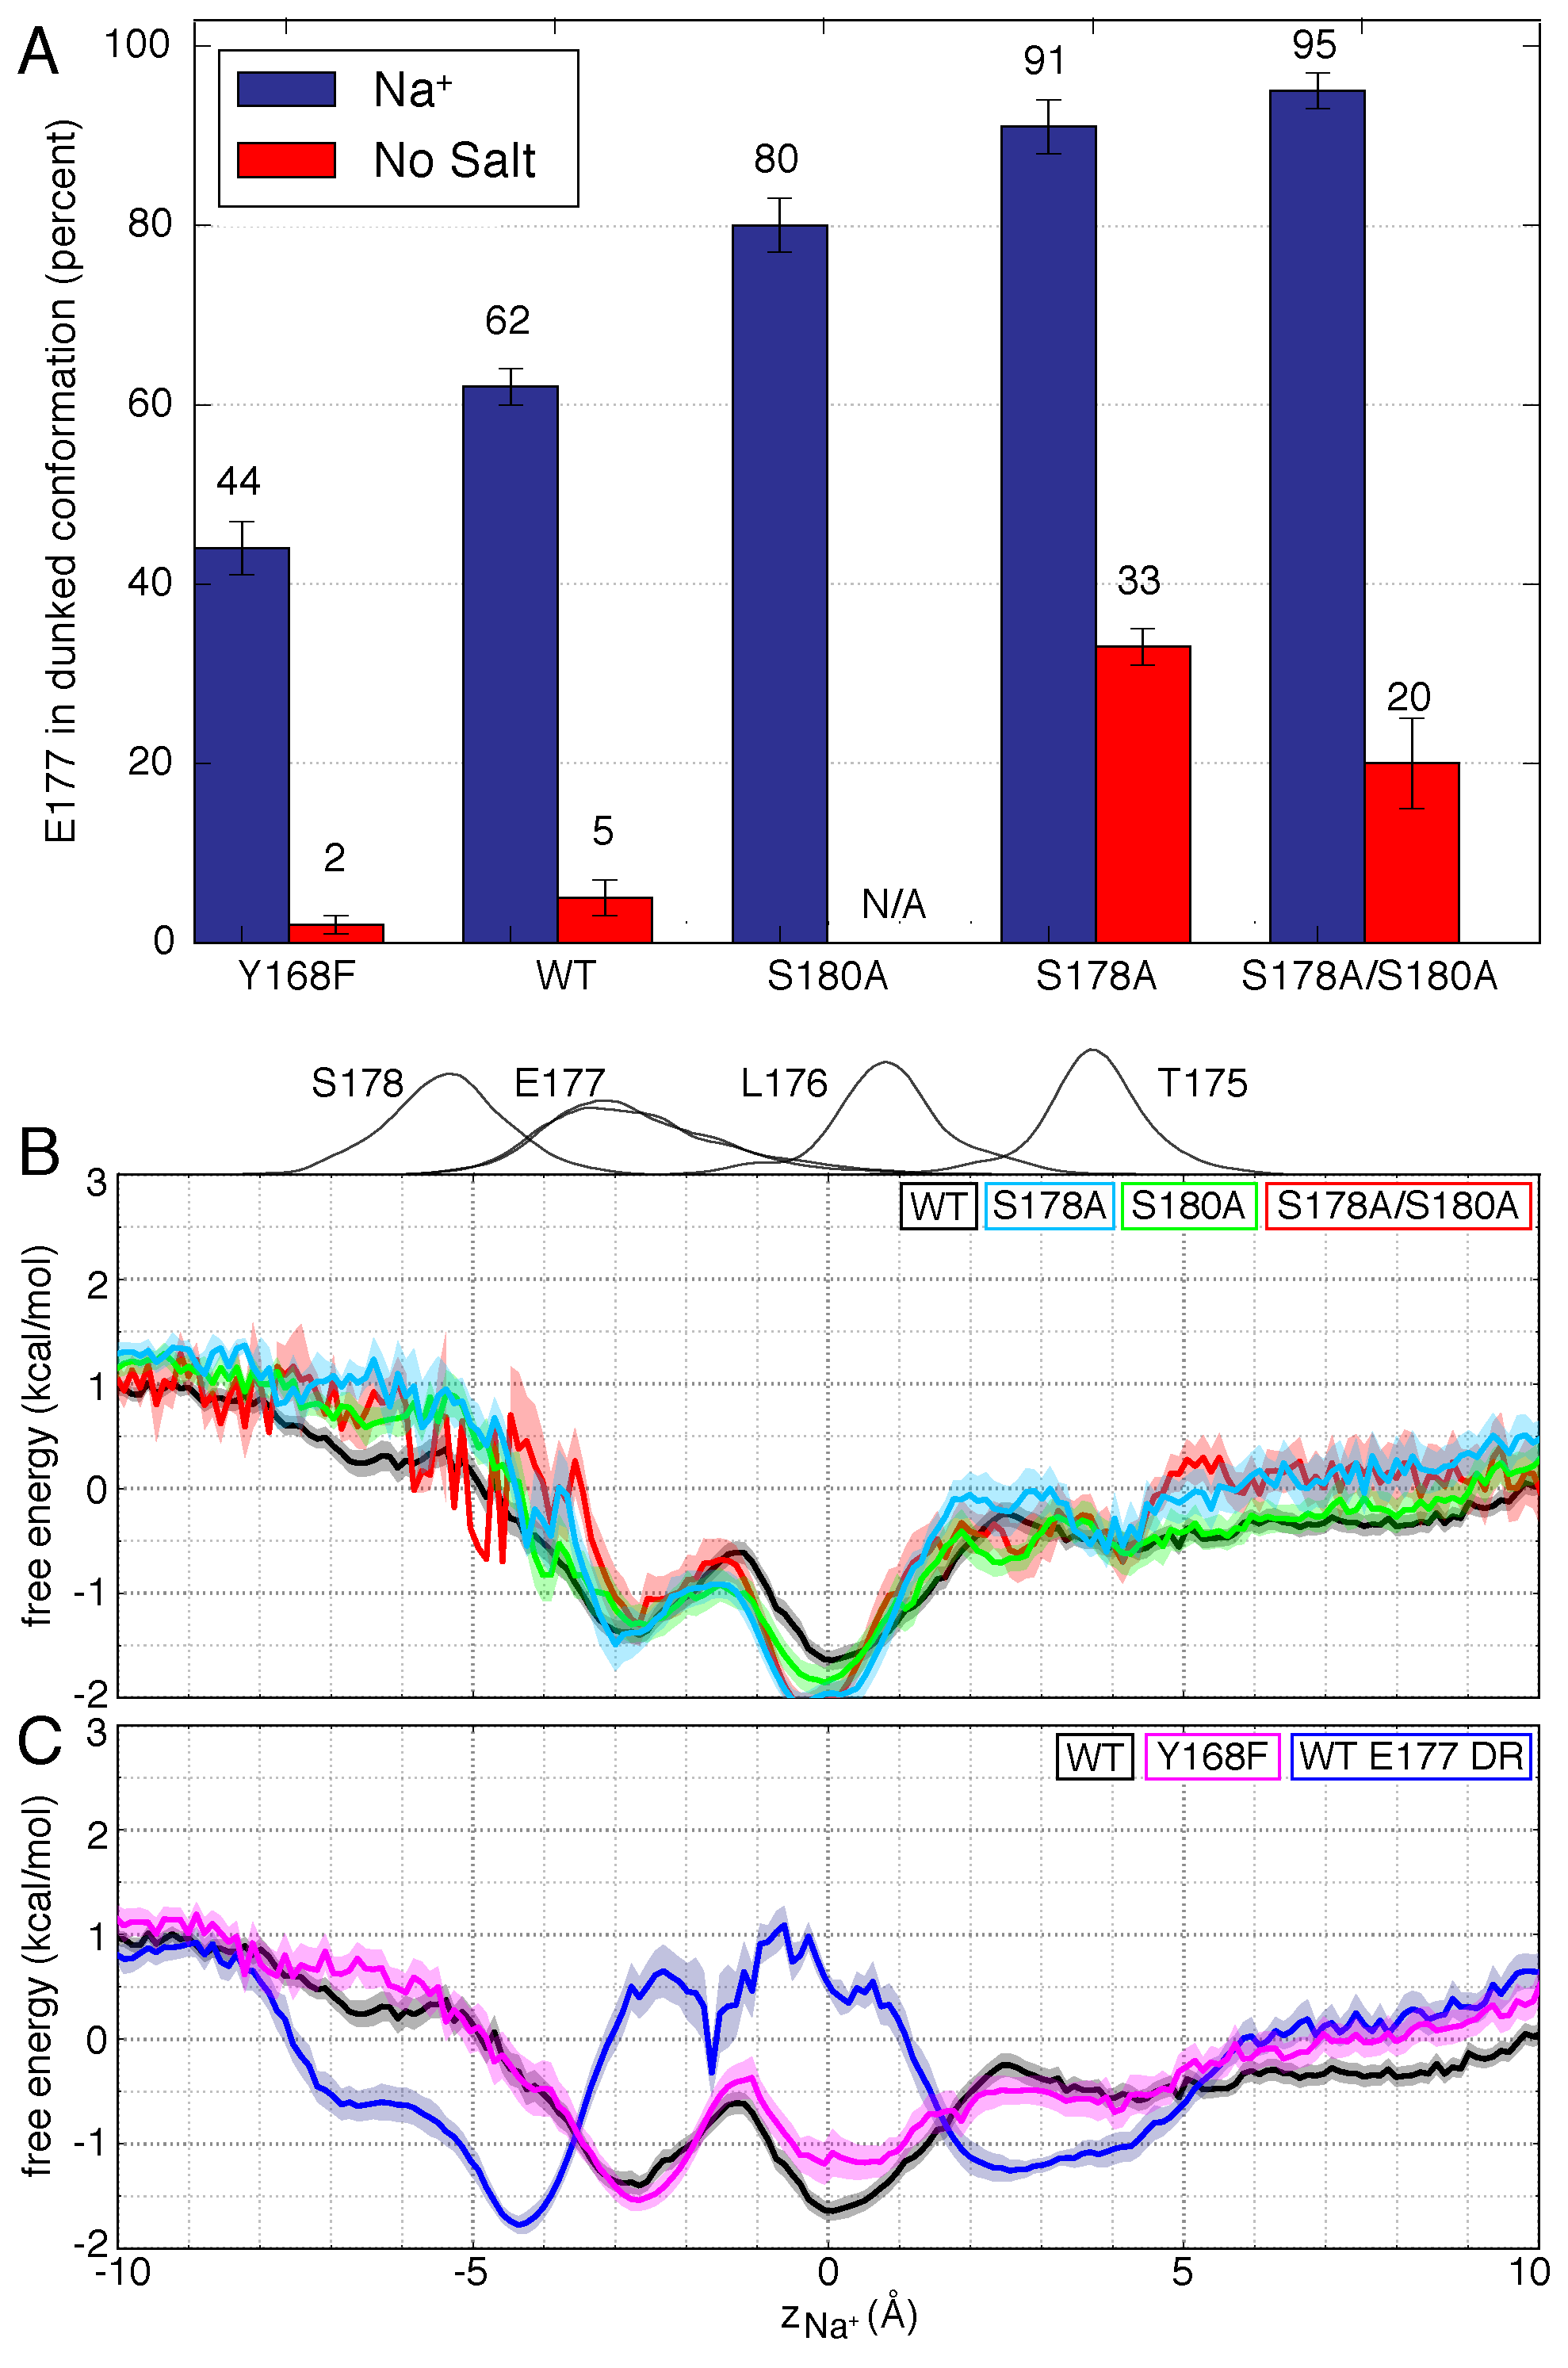
\includegraphics[width=0.7\textwidth]{nav6/Nav6FigS1}
\caption[E177 side chain conformational isomerization and PMF for the movement of Na$^+$ with the OPLS force field]{\textbf{E177 side chain conformational isomerization and PMF for the movement of Na$^+$ with the OPLS force field}. (\textbf{A}) The mean percentage of simulation time in the E177 side chain adopted a lumen-facing state. Data is shown for Y168F, WT, S180A, S178A, and S178A/S180A in the presence of either Na$^+$ (blue) or no ions (red). Error bars are computed as the standard error of mean across all simulation repeats. One-dimensional multi-ion PMFs for Na$^+$ movement along the channel axis in the (\textbf{B}) WT, S178A, S180A, S178A/S180A models. One-dimensional PMFs are also shown for the (\textbf{C}) WT, Y168F, and WT model with E177 dihedral restraints (E177 DR). The reference state (zero free energy) is defined as the bulk extracellular value for Na$^+$ in each dataset separately. The axial distribution of pore-lining oxygen atoms of S178, E177, L176, and T175 are shown from WT simulations above both Na$^+$ and K$^+$ plots.}
\label{fig:nav6figS1}
\end{figure}

We examined the relationship between E177 fluctuations and the multi-ion conduction mechanism using 2D PMFs for distinct ion pairs in the 2 and 3 ion occupancy states (\Cref{fig:nav6figS2,fig:nav6figS3,fig:nav6figS4,fig:nav6figS5,fig:nav6figS6}). This analysis provides information about the preferred positions of ion pairs and greater detail regarding the origin of features in the 1D PMF. With respect to the WT model, the S180A model has a reduced free energy barrier at the site within the SF where ions bind predominately to S178 and E177 with. This axial position corresponds to the location where multiple Na$^+$ have been observed to bind at same axial position (\Cref{fig:nav6figS2,fig:nav6figS3}). The free energy landscape for Na$^+$ is more diffusive for individual ions in the 3 ion state than the 2 ion state, but increased dunking in this mutant does not enhance this effect compared to the WT system. The Na$^+$ free energy surface is flatter than that of K$^+$ throughout the SF, which is common to both S180A and WT models. Increased E177 conformational isomerization in the S180A model appears to have no significant effect on the conduction mechanism within the SF. 

\begin{figure}[!ptb]
\centering
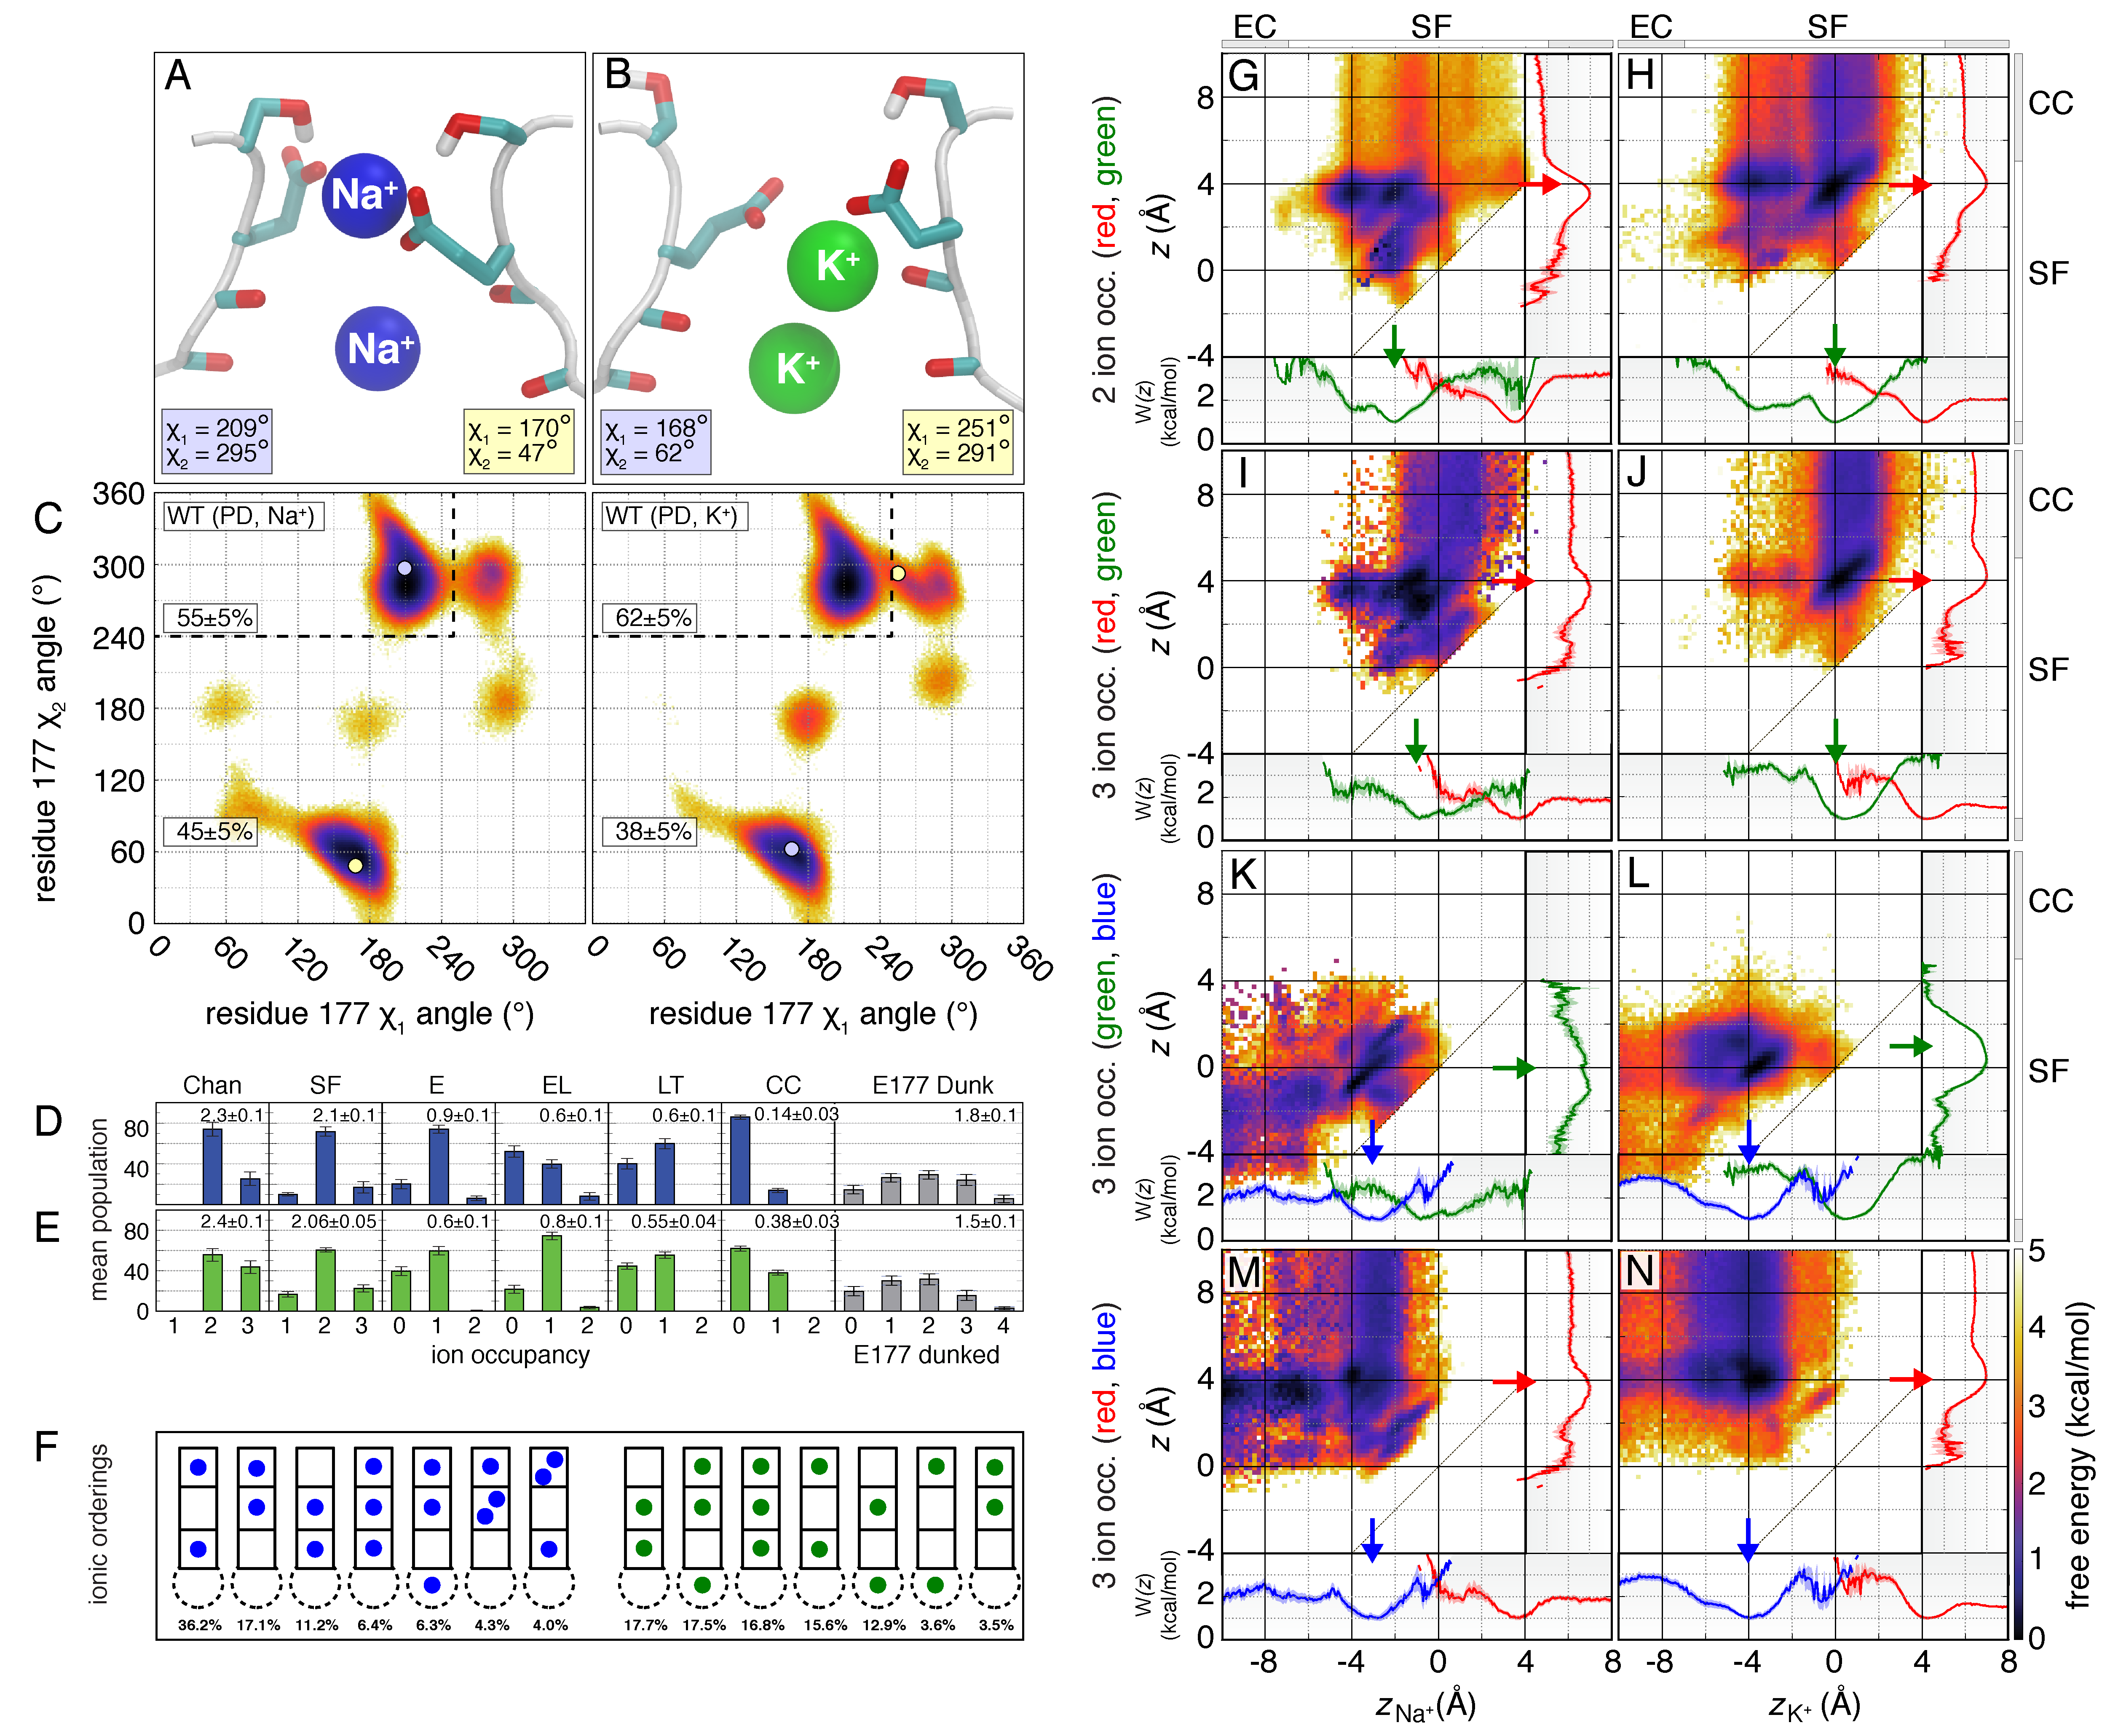
\includegraphics[width=0.8\textwidth]{nav6/Nav6FigS2}
\caption[Binding statistics and potential of mean-force (PMF) for the movement of Na$^+$ and K$^+$ along the channel axis in the WT PD model]{\textbf{Binding statistics and potential of mean-force (PMF) for the movement of Na$^+$ and K$^+$ along the channel axis in the WT PD model}. (\textbf{A-B}) Representative snapshots of the SF for high population ionic configurations in the presence of Na$^+$ and K$^+$, with E177 sidechain $\chi_1$ and $\chi_2$ angles shown for both left (purple) and right (yellow) subunits. (\textbf{B}) Population of E177 side chain torsions ($\chi_1$, $\chi_2$) across all WT simulation data for Na$^+$ and K$^+$. ($\chi_1$, $\chi_2$) pairs are shown as yellow and purple dots in correspondence with the left and right subunits in (A-B), respectively. A dashed line separates the crystallographic E177 side chain configuration and the lumen-facing conformation, with total state populations shown within each region. Ionic occupancy of the entire channel and SF, as well as specific `E', `EL', `LT', and `CC' binding sites, as well as the distribution of number of dunked E177 side chains, for (\textbf{D}) Na$^+$ and (\textbf{E}) K$^+$. (\textbf{F}) The seven highest population ionic configurations with the channel for Na$^+$ and K$^+$, where the four primary binding sites are identified as `E', `EL', `LT', and `CC' from top to bottom. Two-dimensional potential of mean-force (PMF) for (\textbf{G, I, K, M}) Na$^+$ and (\textbf{H, J, L, N}) K$^+$ pairs along the channel axis. Ions are ranked by axial position from CC to EC with the colors `red', `green', and `blue' for both ion types. PMFs for Na$^+$ and K$^+$ are computed between ion pairs for channel occupancy states; (\textbf{G,H}) 2 and (\textbf{I-N}) 3. For three ion occupancy, all distinct two ion pairs are plotted. On all 2D PMFs a one-dimensional projection of the axial free energy for each ion are shown on the vertical and horizontal axes and are colored for the target ion (identified with colored arrows). The reference state (zero free energy) of each panel is set to the highest probability microstate within each channel occupancy state sub-ensemble, which applies to all subsequent ion pair 2D PMFs.}
\label{fig:nav6figS2}
\end{figure}

\begin{figure}[!ptb]
\centering
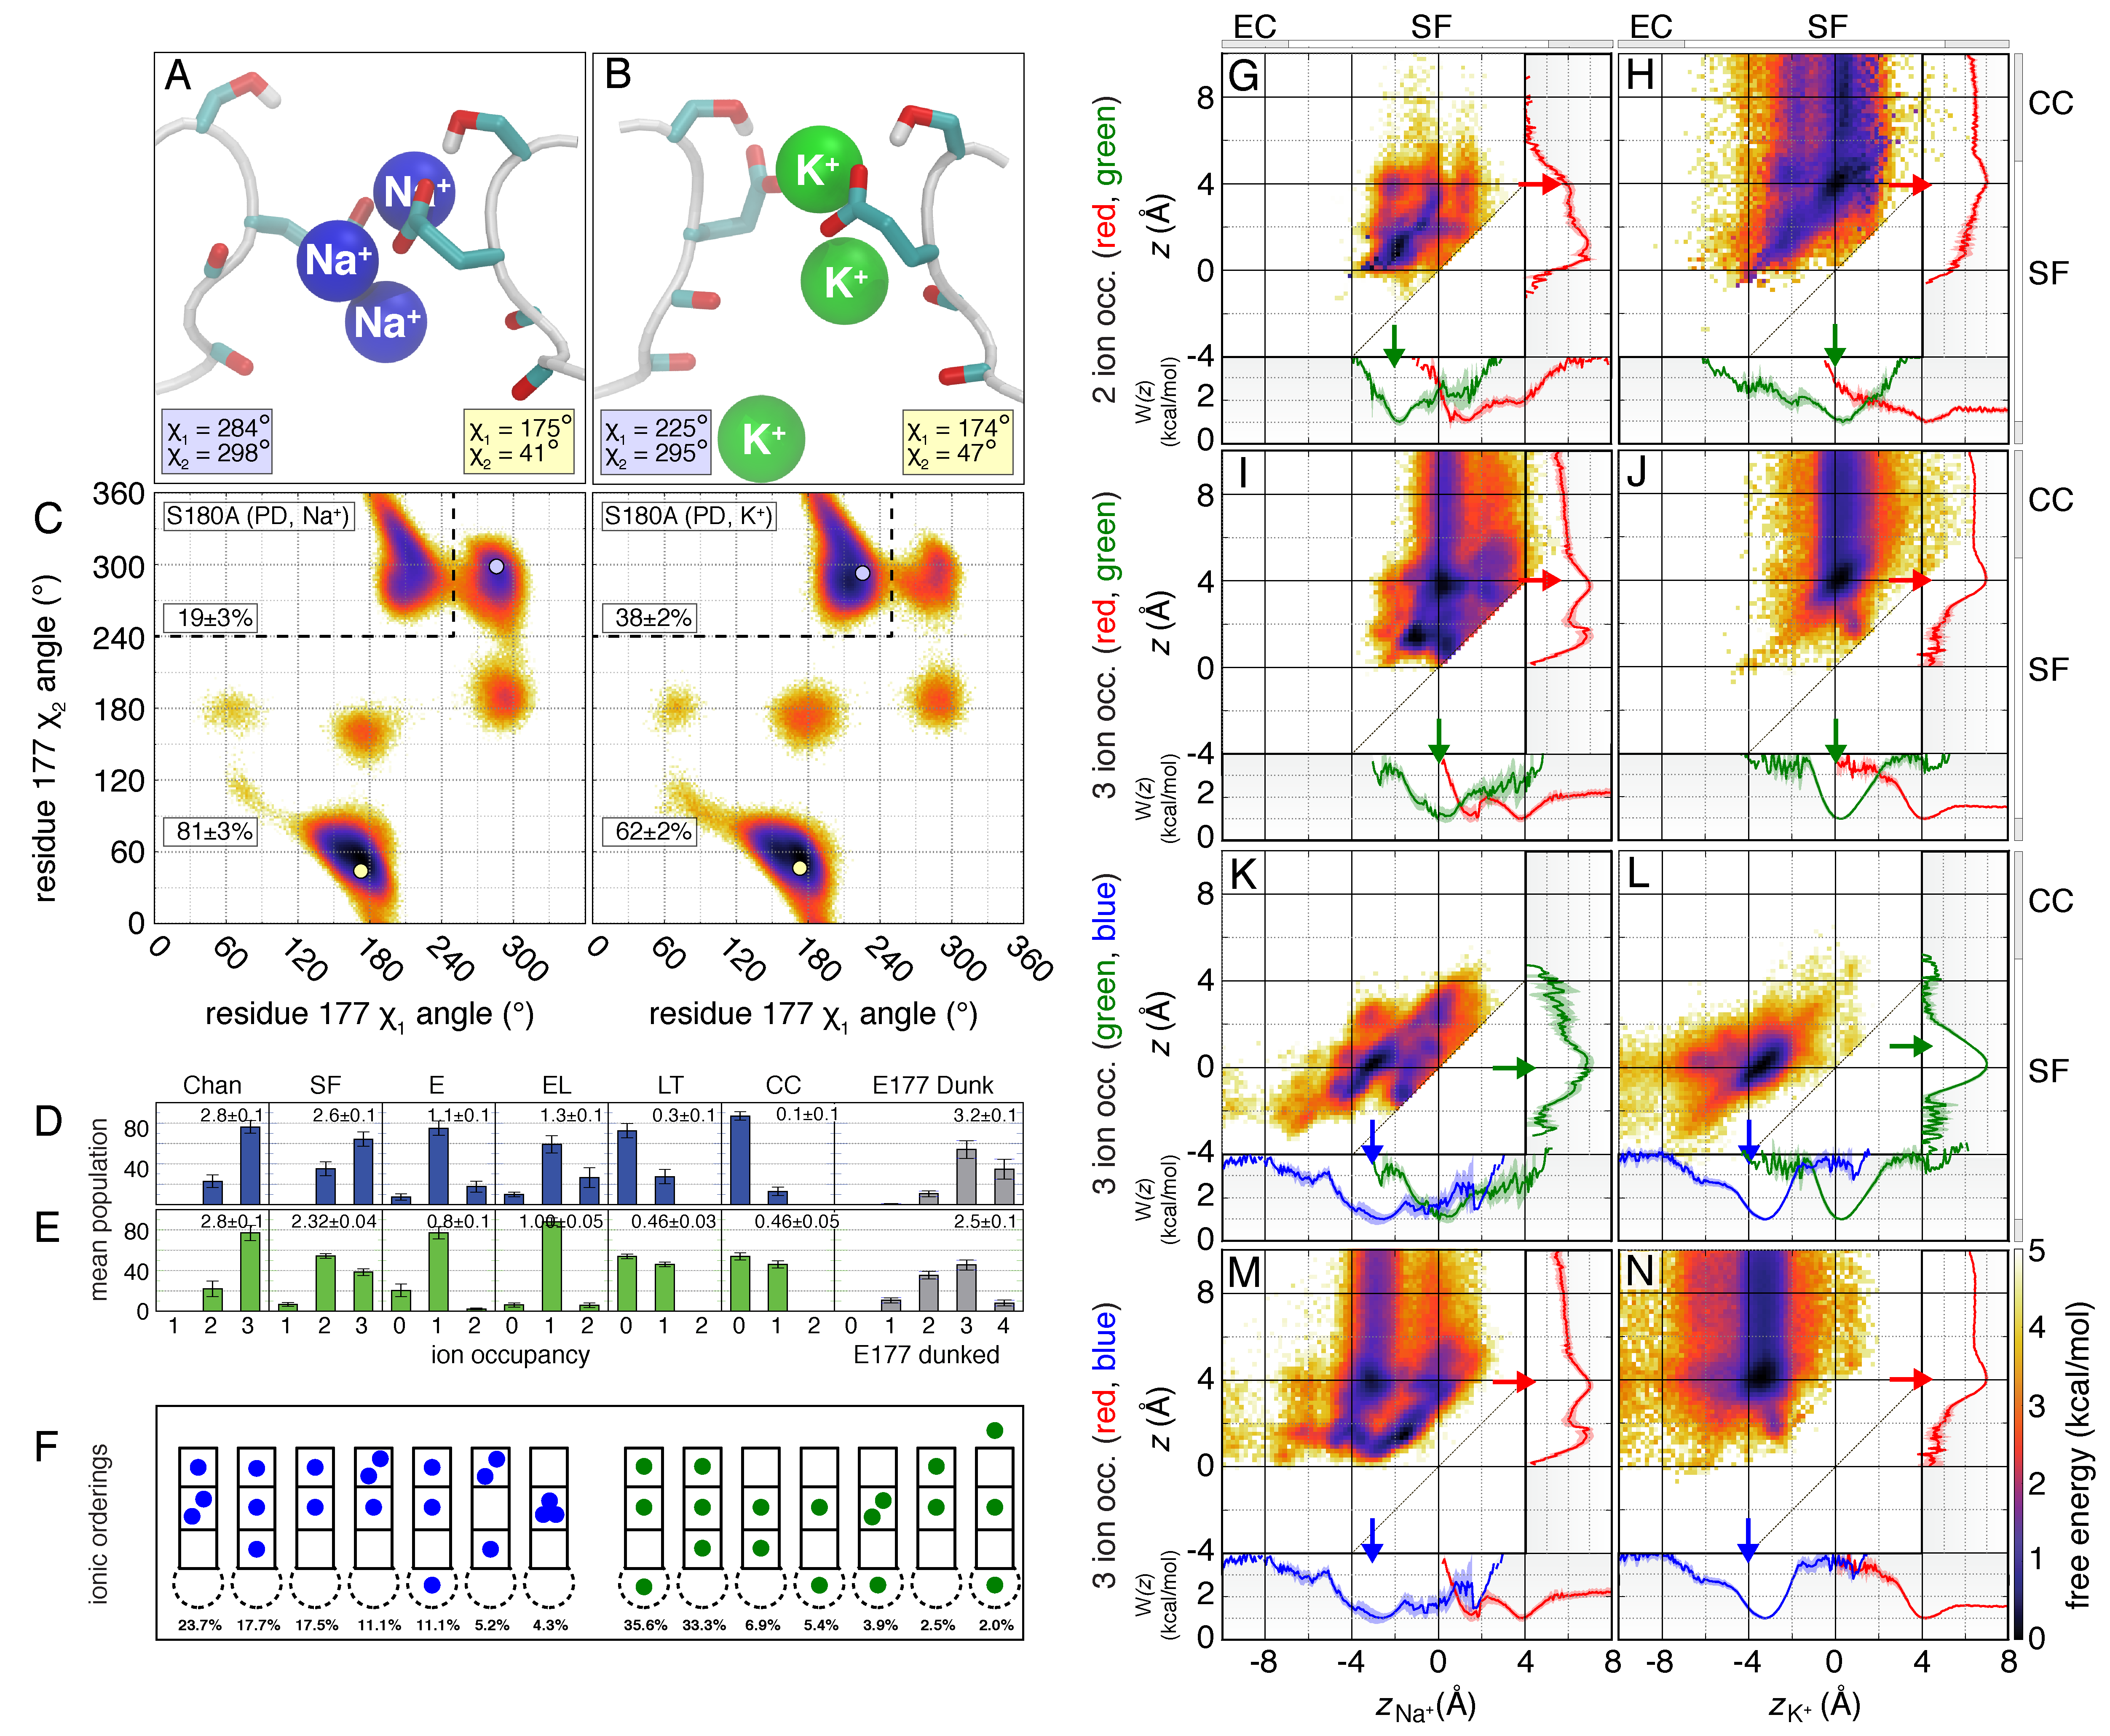
\includegraphics[width=0.8\textwidth]{nav6/Nav6FigS3}
\caption[Binding statistics and potential of mean-force (PMF) for the movement of Na$^+$ and K$^+$ along the channel axis in the S180A PD model]{ \textbf{Binding statistics and potential of mean-force (PMF) for the movement of Na$^+$ and K$^+$ along the channel axis in the S180A PD model}. (\textbf{A-B}) Representative snapshots of the SF for high population ionic configurations in the presence of Na$^+$ and K$^+$. (\textbf{C}) Population of E177 side chain torsions ($\chi_1$, $\chi_2$) across all S180A simulation data for Na$^+$ and K$^+$. Ionic occupancy of the entire channel and SF, as well as specific `E', `EL', `LT', and `CC' binding sites, as well as the distribution of number of dunked E177 side chains, for (\textbf{D}) Na$^+$ and (\textbf{E}) K$^+$. (\textbf{F}) The seven highest population ionic configurations with the channel for Na$^+$ and K$^+$, where the four primary binding sites are identified as `E', `EL', `LT', and `CC' from top to bottom. Two-dimensional potential of mean-force (PMF) for (\textbf{G, I, K, M}) Na$^+$ and (\textbf{H, J, L, N}) K$^+$ pairs along the channel axis. PMFs for Na$^+$ and K$^+$ are computed between ion pairs for channel occupancy states; (\textbf{G, H}) 2 and (\textbf{I-N}) 3. For three ion occupancy, all distinct two ion pairs are plotted. For more information, refer to the caption of Figure \ref{fig:nav6figS2}.}
\label{fig:nav6figS3}
\end{figure}

In the S178A and S178A/S180A models, concerted motion of ion pairs appears reduced in both 2 and 3 ion occupancy states due to reduced binding at the `E' site at $\approx$-4 \AA (\Cref{fig:nav6figS4,fig:nav6figS5}). However, in both ion occupancy states, dual occupancy of the `E' binding site by Na$^+$ and K$^+$ is increased relative to the WT channel, suggesting that the molecular mechanism of conduction is perturbed. As a result of this change in the outer binding site of the SF, Na$^+$ and K$^+$ bind in similar ways within the SF, having outer and central ion binding sites shifted to the intracellular side of the SF compared to the WT model. These Ser-to-Ala models have a higher propensity for Na$^+$ and K$^+$ binding at the same axial position compared to the WT model. The free energy barrier for K$^+$ at position $\approx -2$ \AA is not strongly present in S178A and S178A/S180A models, suggesting that Na$^+$ selectivity is impaired. 

\begin{figure}[!ptb]
\centering
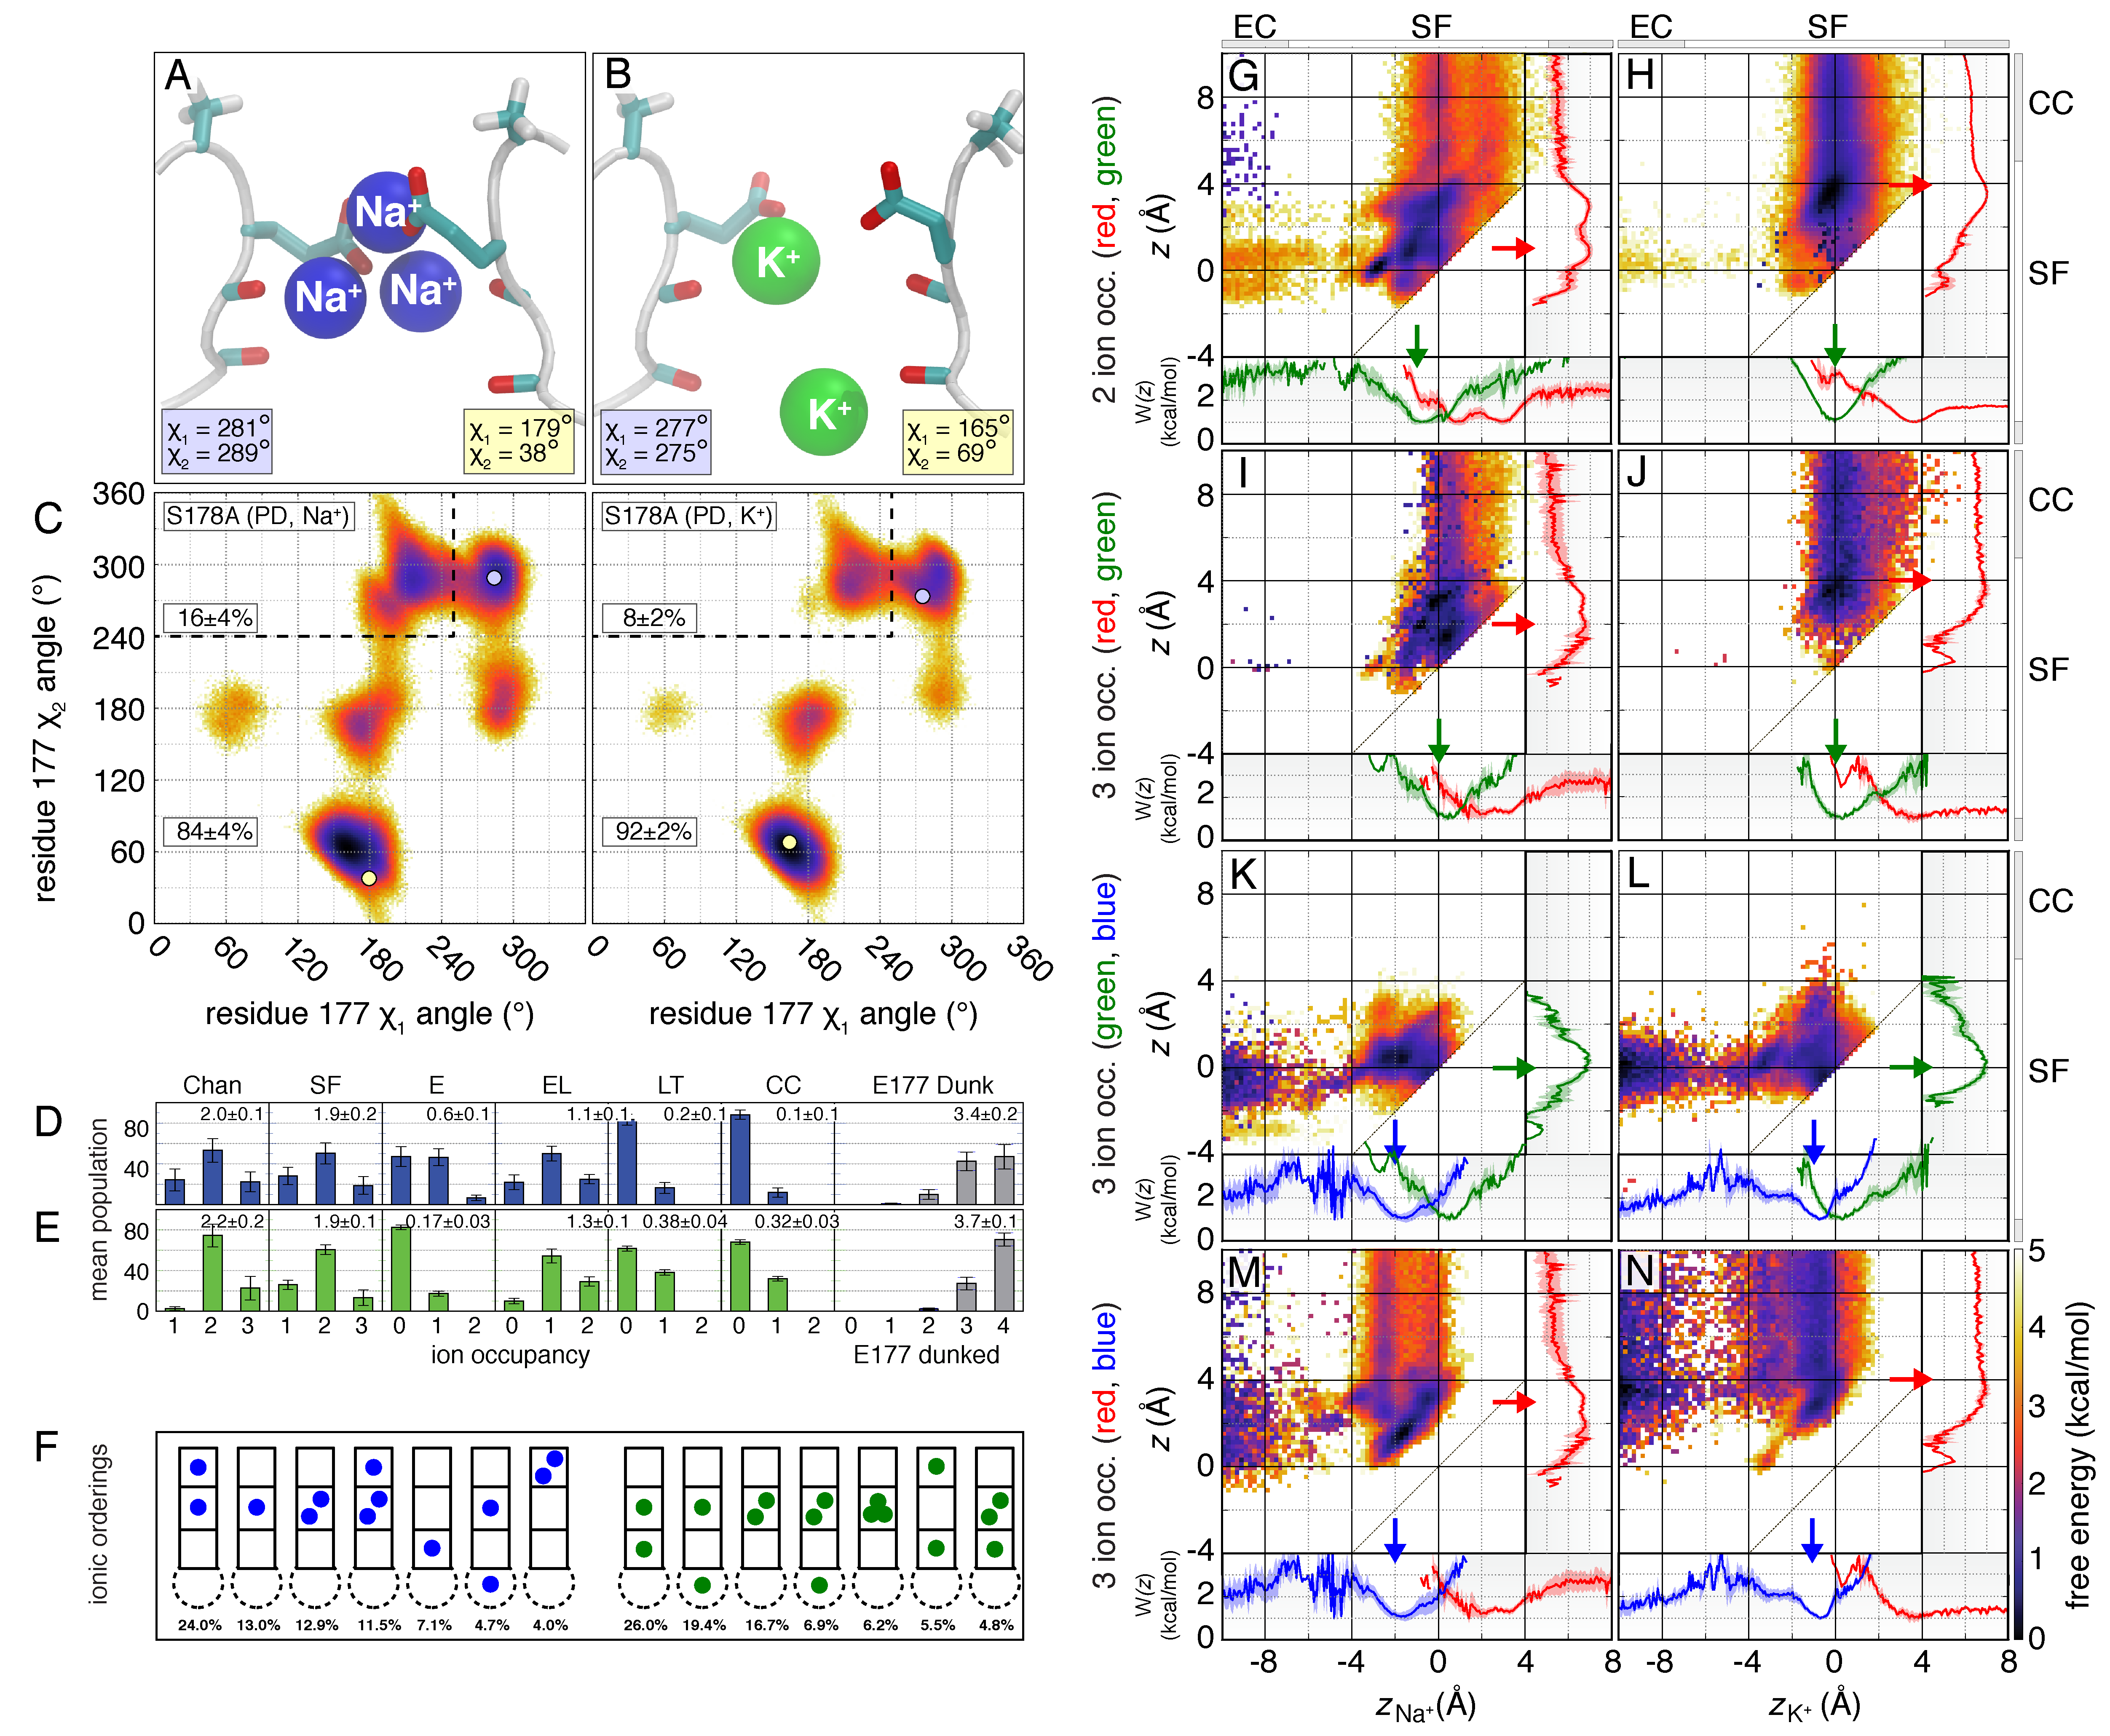
\includegraphics[width=0.8\textwidth]{nav6/Nav6FigS4}
\caption[Binding statistics and potential of mean-force (PMF) for the movement of Na$^+$ and K$^+$ along the channel axis in the S178A PD model]{ \textbf{Binding statistics and potential of mean-force (PMF) for the movement of Na$^+$ and K$^+$ along the channel axis in the S178A PD model}. (\textbf{A-B}) Representative snapshots of the SF for high population ionic configurations in the presence of Na$^+$ and K$^+$. (\textbf{C}) Population of E177 side chain torsions ($\chi_1$, $\chi_2$) across all S178A simulation data for Na$^+$ and K$^+$. Ionic occupancy of the entire channel and SF, as well as specific `E', `EL', `LT', and `CC' binding sites, as well as the distribution of number of dunked E177 side chains, for (\textbf{D}) Na$^+$ and (\textbf{E}) K$^+$. (\textbf{F}) The seven highest population ionic configurations with the channel for Na$^+$ and K$^+$, where the four primary binding sites are identified as `E', `EL', `LT', and `CC' from top to bottom. Two-dimensional potential of mean-force (PMF) for (\textbf{G, I, K, M}) Na$^+$ and (\textbf{H, J, L, N}) K$^+$ pairs along the channel axis. PMFs for Na$^+$ and K$^+$ are computed between ion pairs for channel occupancy states; (\textbf{G, H}) 2 and (\textbf{I-N}) 3. For three ion occupancy, all distinct two ion pairs are plotted. For more information, refer to the caption of Figure \ref{fig:nav6figS2}.}
\label{fig:nav6figS4}
\end{figure}

\begin{figure}[!ptb]
\centering
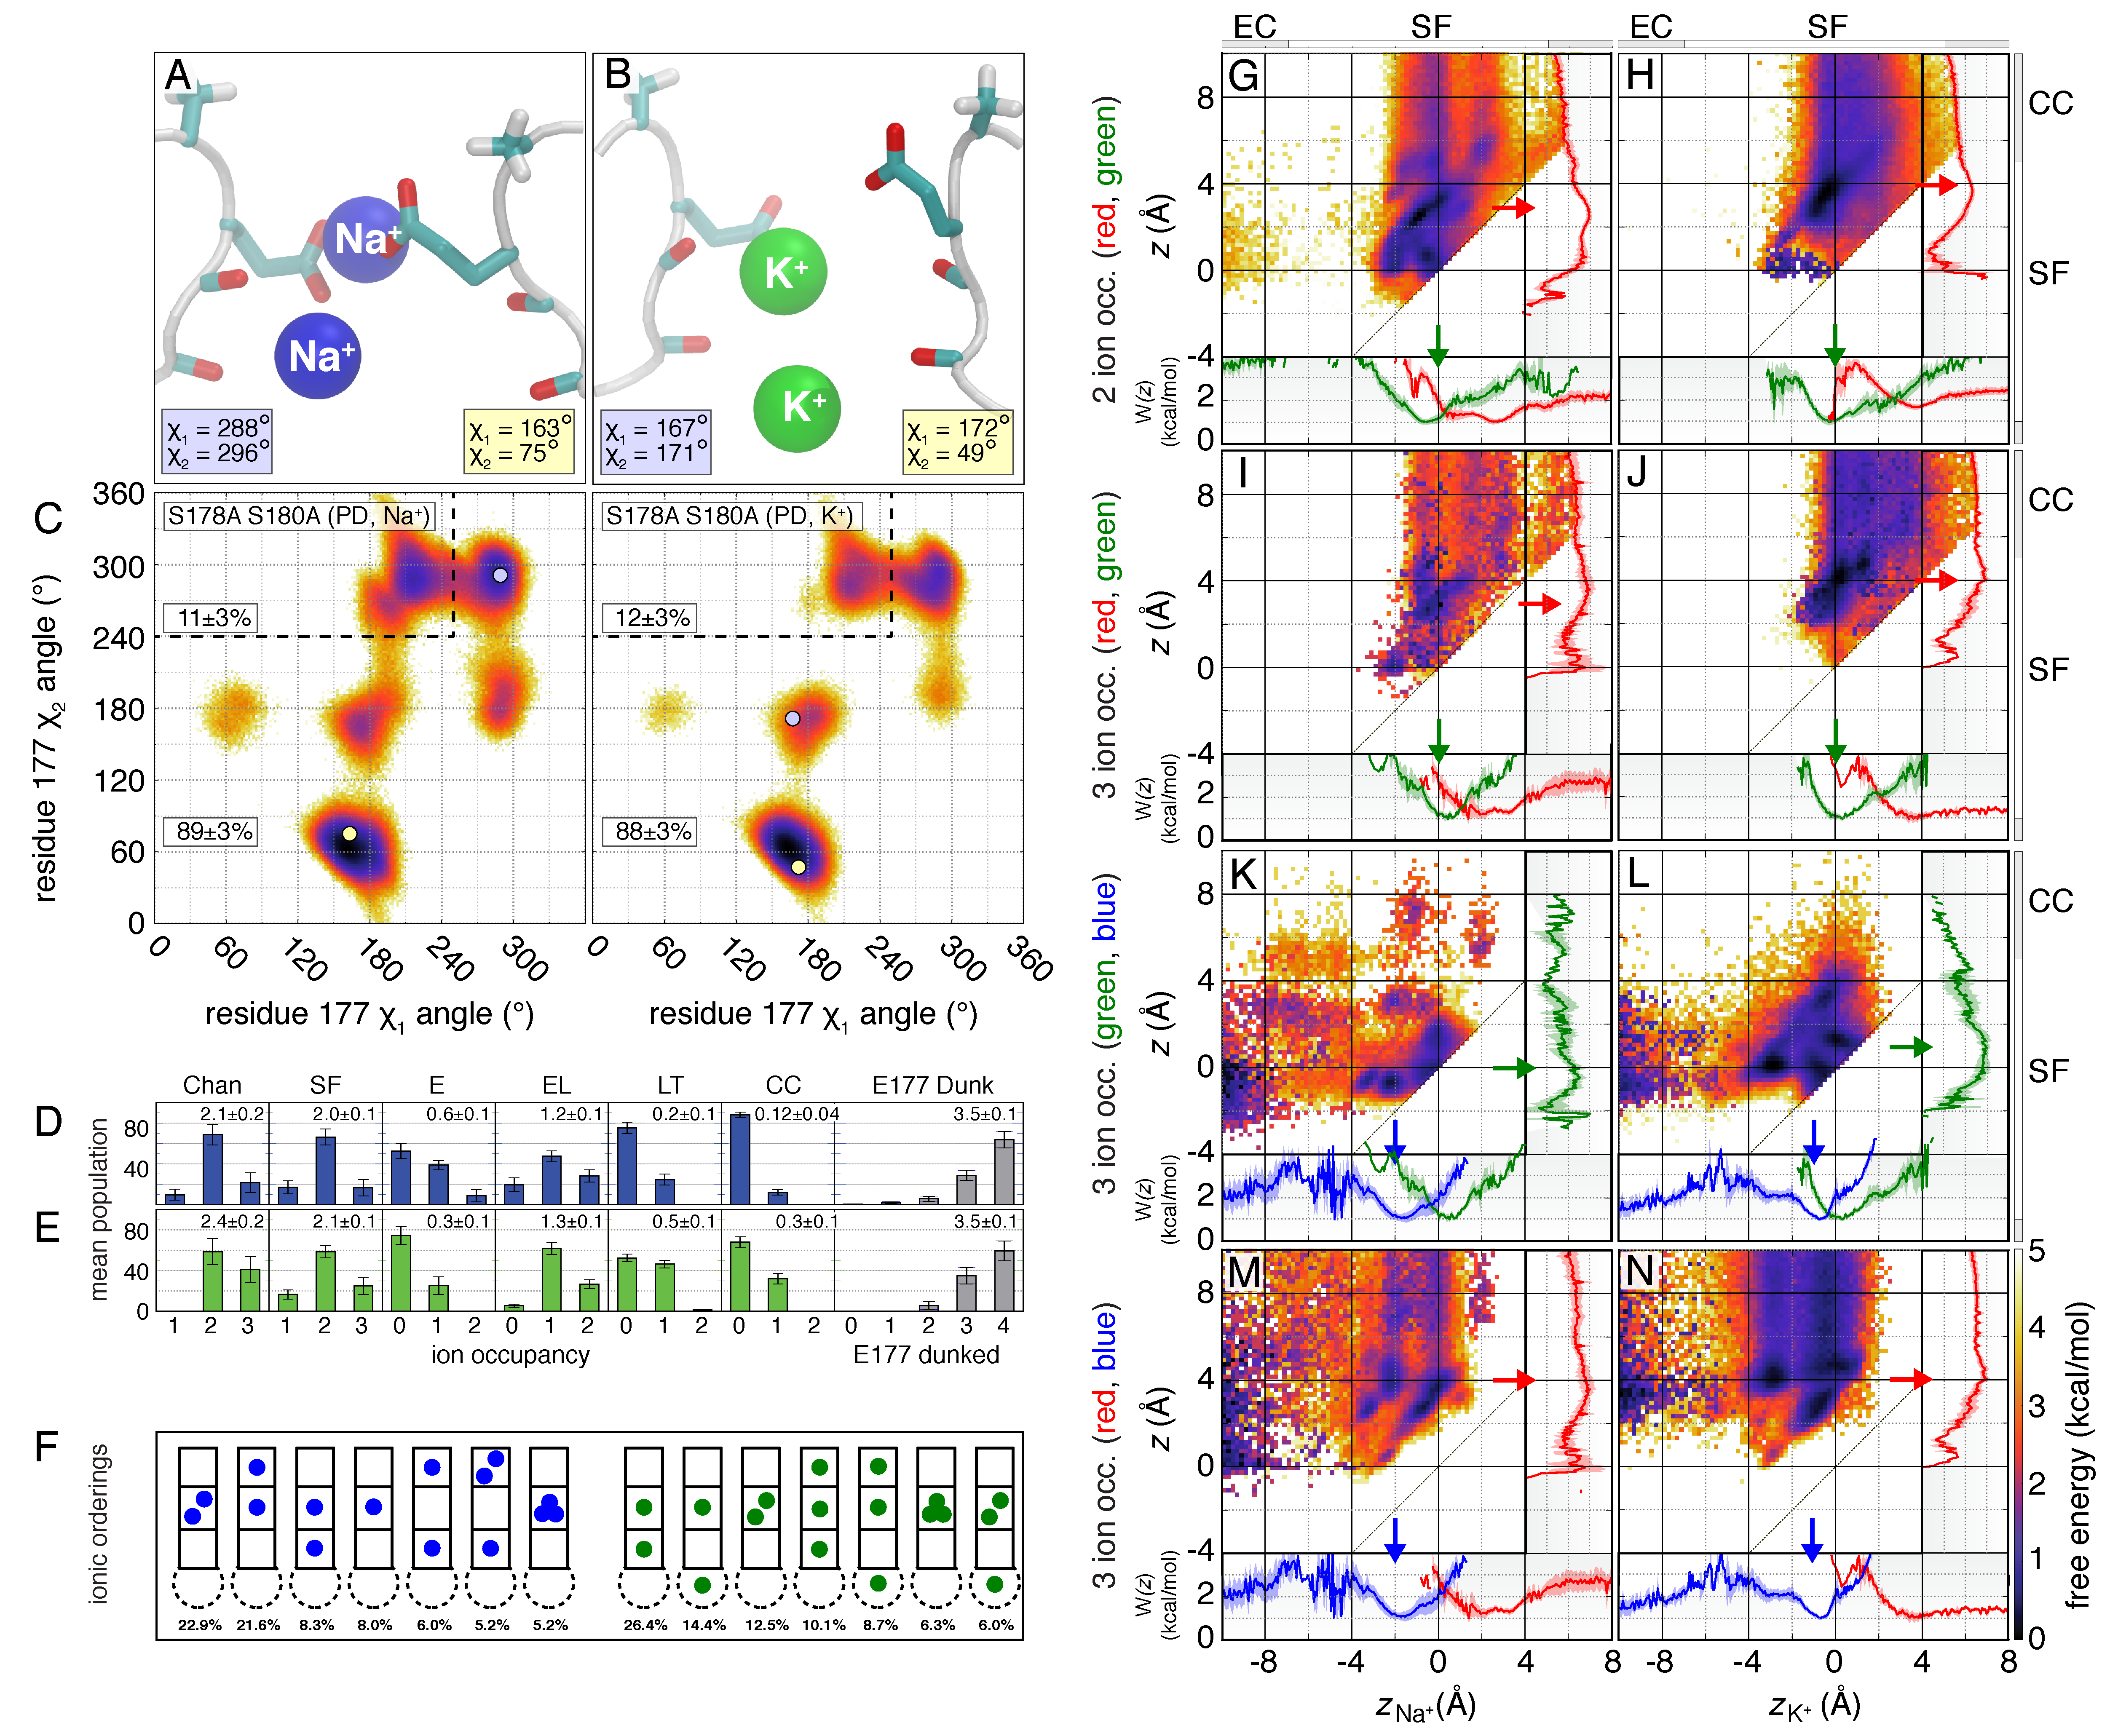
\includegraphics[width=0.8\textwidth]{nav6/Nav6FigS5}
\caption[Binding statistics and potential of mean-force (PMF) for the movement of Na$^+$ and K$^+$ along the channel axis in the S178A/S180A PD model]{ \textbf{Binding statistics and potential of mean-force (PMF) for the movement of Na$^+$ and K$^+$ along the channel axis in the S178A/S180A PD model}. (\textbf{A-B}) Representative snapshots of the SF for high population ionic configurations in the presence of Na$^+$ and K$^+$. (\textbf{C}) Population of E177 side chain torsions ($\chi_1$, $\chi_2$) across all S178A/S180A simulation data for Na$^+$ and K$^+$. Ionic occupancy of the entire channel and SF, as well as specific `E', `EL', `LT', and `CC' binding sites, as well as the distribution of number of dunked E177 side chains, for (\textbf{D}) Na$^+$ and (\textbf{E}) K$^+$. (\textbf{F}) The seven highest population ionic configurations with the channel for Na$^+$ and K$^+$, where the four primary binding sites are identified as `E', `EL', `LT', and `CC' from top to bottom. Two-dimensional potential of mean-force (PMF) for (\textbf{G, I, K, M}) Na$^+$ and (\textbf{H, J, L, N}) K$^+$ pairs along the channel axis. PMFs for Na$^+$ and K$^+$ are computed between ion pairs for channel occupancy states; (\textbf{G, H}) 2 and (\textbf{I-N}) 3. For three ion occupancy, all distinct two ion pairs are plotted. For more information, refer to the caption of Figure \ref{fig:nav6figS2}.}
\label{fig:nav6figS5}
\end{figure}

In the dunking reduced Y168F model, there is a dramatic alteration of Na$^+$ binding and mobility. Na$^+$ and K$^+$ preferentially adopt a single-file 2 ion state at `E' and `LT' sites (Fig. \ref{fig:nav6figS6}). In both cases Na$^+$ rarely adopts the `LT' site, but K$^+$ is capable of doing so along with a higher likelihood of concerted motion. Based on these results, we would expect that Na$^+$ selectivity is also impaired or potentially reversed in favour of K$^+$. The concerted and knock-on conduction mechanisms are significantly disrupted for Na$^+$ in this model, and are nearly identical to the E177 DR system. Together, these results provide a foundation for experimental validation of the role of channel fluctuations in conduction and selectivity in Nav channels.

\begin{figure}[!ptb]
\centering
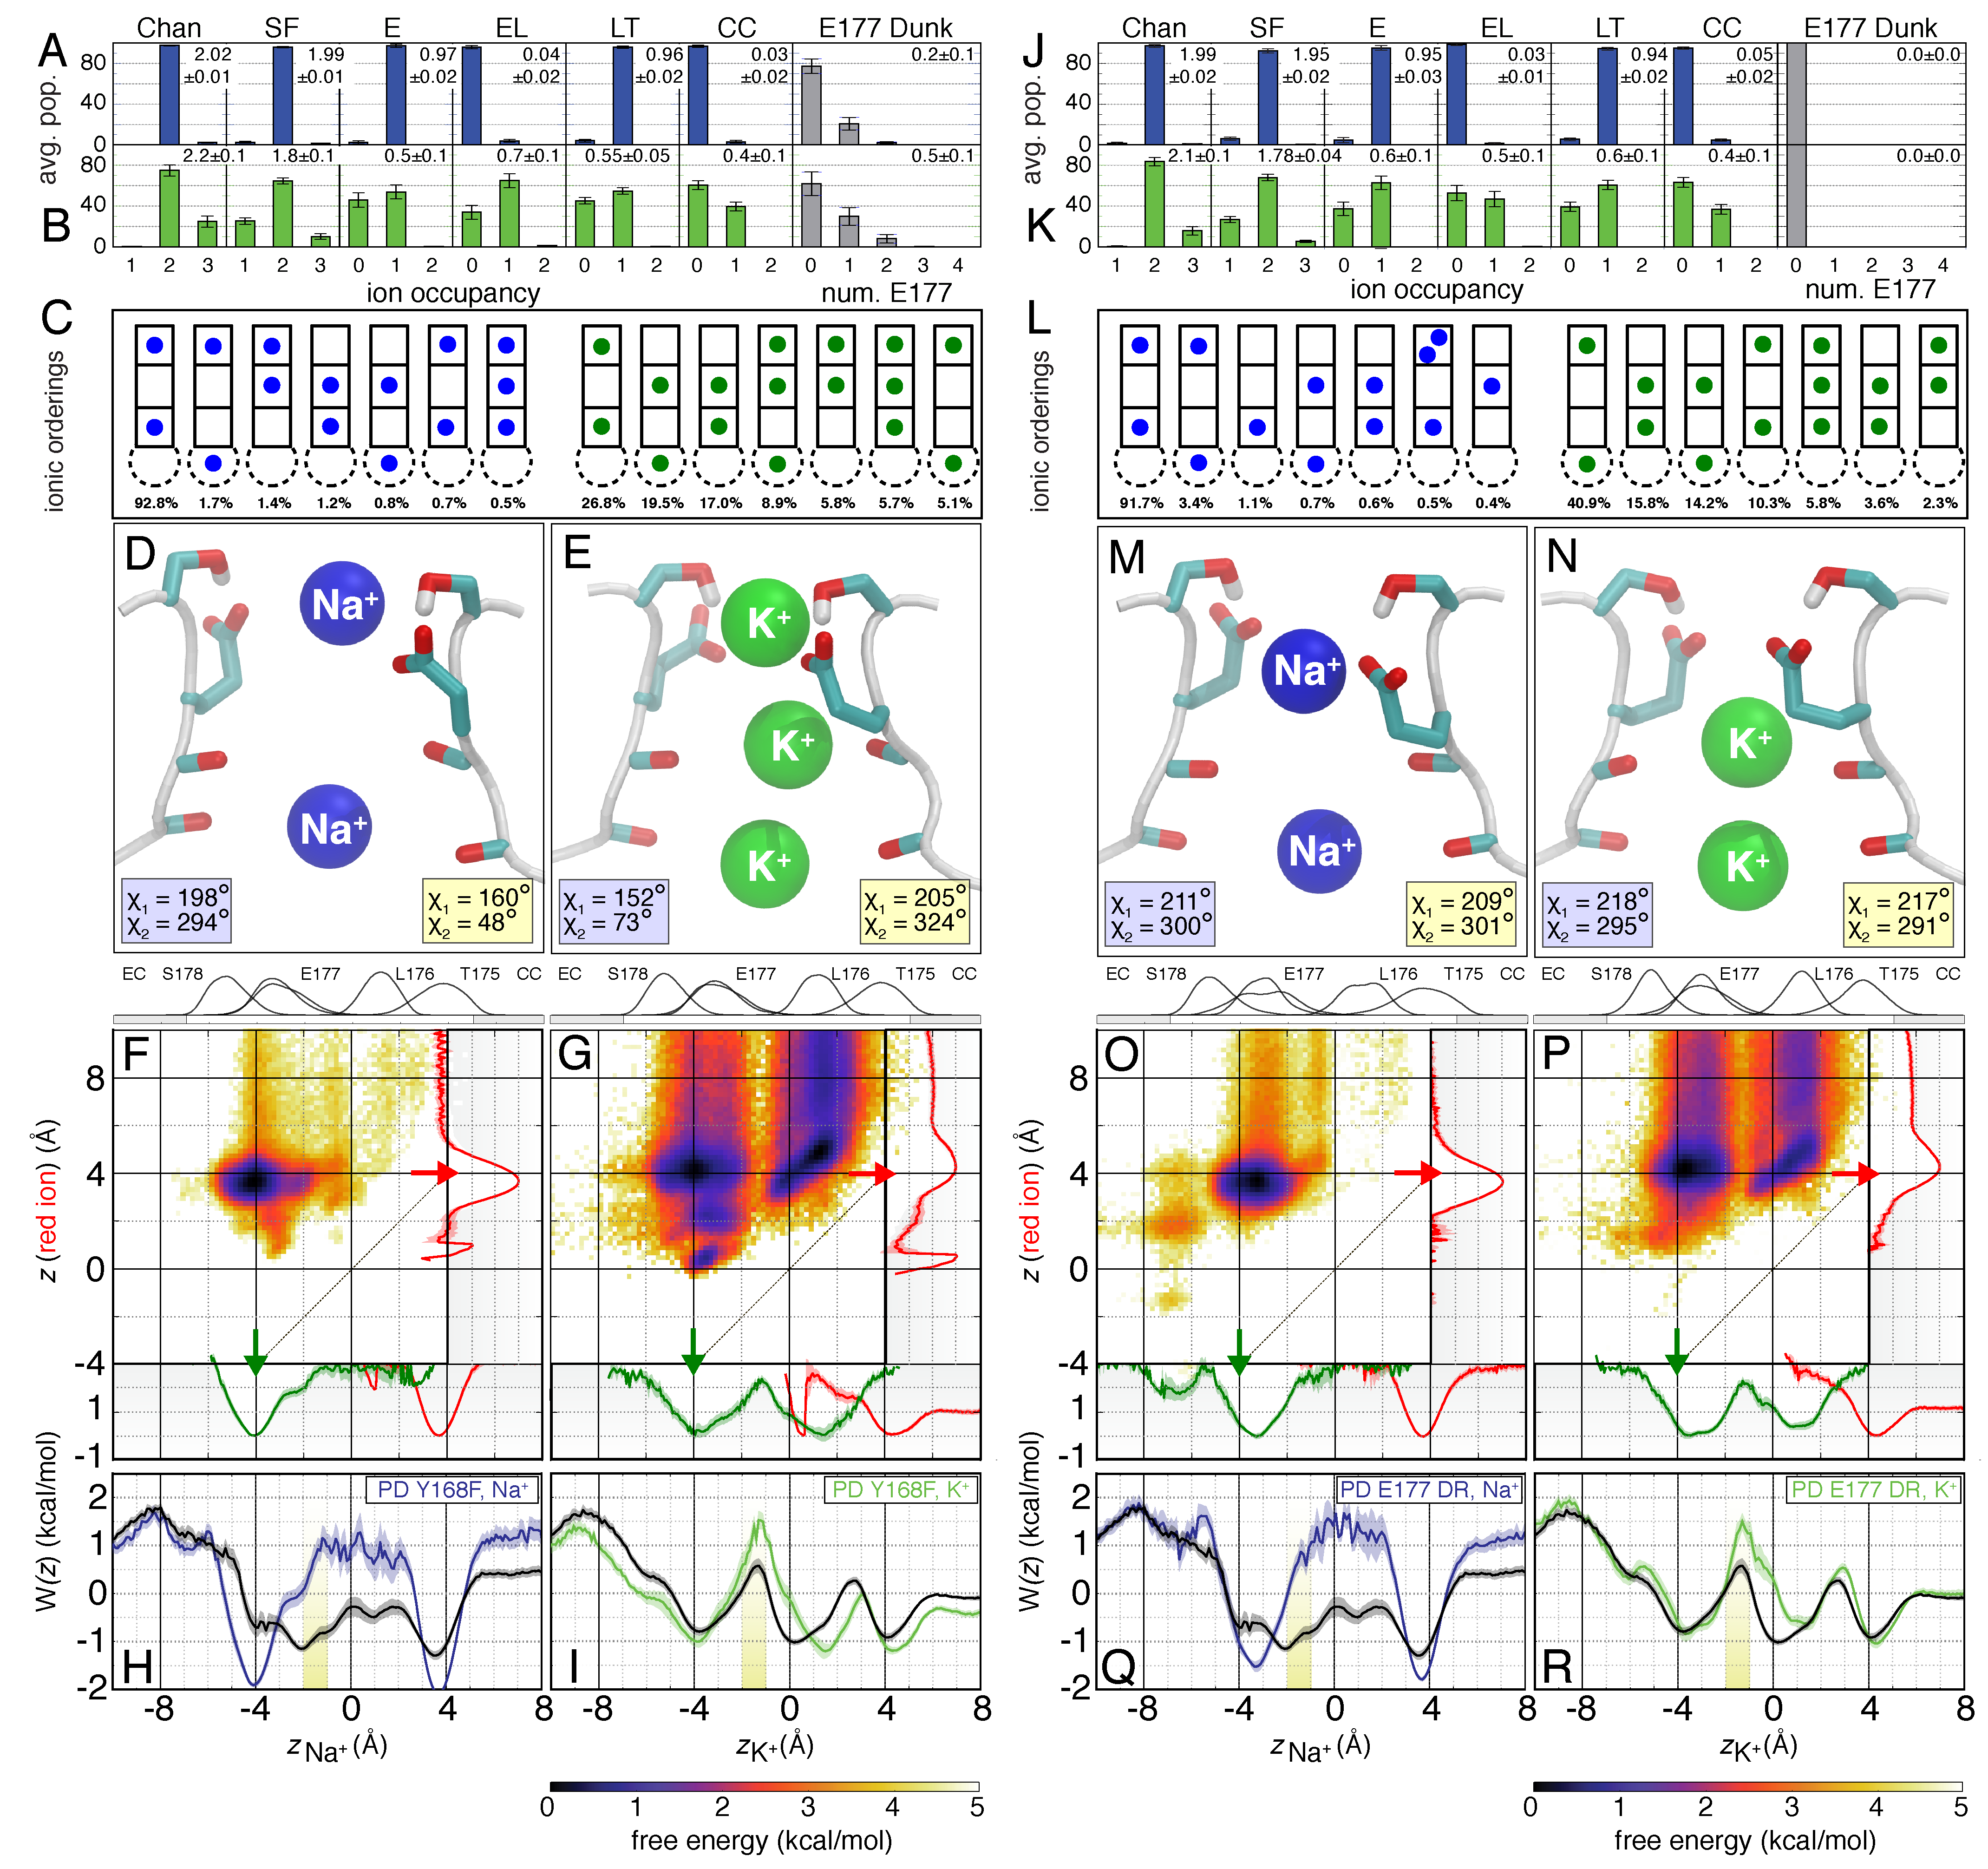
\includegraphics[width=0.8\textwidth]{nav6/Nav6FigS6}
\caption[Binding statistics and potential of mean-force (PMF) for the movement of Na$^+$ and K$^+$ along the channel axis in the Y168F and E177DR PD model]{ \textbf{Binding statistics and potential of mean-force (PMF) for the movement of Na$^+$ and K$^+$ along the channel axis in the Y168F and E177DR PD model}. Ionic occupancy of the entire channel and SF, as well as specific `E', `EL', `LT', and `CC' binding sites, as well as the distribution of number of dunked E177 side chains, for (\textbf{A}) Na$^+$ and (\textbf{B}) K$^+$. (\textbf{C}) The seven highest population ionic configurations with the channel for Na$^+$ and K$^+$, where the four primary binding sites are identified as `E', `EL', `LT', and `CC' from top to bottom. (\textbf{D-E}) Representative snapshots of the SF for high population ionic configurations in the presence of Na$^+$ and K$^+$. Two-dimensional potential of mean-force (PMF) for (\textbf{F}) Na$^+$ and (\textbf{G}) K$^+$ pairs along the channel axis for the two ion occupancy state. The multi-ion 1D PMF for (\textbf{H}) Na$^+$ and (\textbf{I}) K$^+$ movement is shown for the Y168F model (blue/green colored lines) as well as the WT model (black line) for reference. Identical plots are shown for the E177 dihedral restrained model (\textbf{J-R}).For more information, refer to the caption of Figure \ref{fig:nav6figS2}.}
\label{fig:nav6figS6}
\end{figure}

\section{Discussion}
Previous molecular simulations suggest that conformational isomerization of glutamic acid side chains in the SF of bacterial voltage-gated sodium channels plays a dual role of catalyzing Na$^+$ conduction and imparting Na$^+$ over K$^+$ selectivity (Chapters 4-5, \cite{Chakrabarti:2013kd}). Here we extend these findings by presenting a set of single-point mutations that displace the conformational equilibrium of E177. The propensity of E177 dunking was linked to quantitative changes in the free-energy of Na$^+$ and K$^+$ conduction. In the S180A mutant, Na$^+$ movement was made more diffusive through the SF, while K$^+$ movement was unaffected. In the S178A and S178A/S180A models, the free energy of Na$^+$ and K$^+$ conduction was similar. Lastly, in the Y168F mutant, Na$^+$ conduction through the SF was blocked, while free energy barriers for K$^+$ increased, but were still surmountable.

These results provide the basis for electrophysiological validation of the hypothesis that E177 dunking is fundamental to conduction and selectivity. Differences in the multi-ion conduction mechanism for Na$^+$ and K$^+$ with respect to the WT channel are expected to result in perturbations to single-channel conductance and electrophysiological measurements of selectivity. Quantitative estimates of conductance and selectivity in voltage-gated cation channels are challenging to compute using molecular simulations \cite{Jensen:2013gn}, and cannot be reliably computed in a closed-channel model, but nonetheless, our results lead to specific predictions. In broad terms, we hypothesize that increased dunking by means of mutations like S180A will increase Na$^+$ conductance and, conversely, decreased dunking by means of the Y168F mutation should decrease conductance. Our confidence in this relationship is stronger for the Y to F mutation, which has a dramatic effect on the dunking propensity and free energy of ion conduction. Based on our previous studies of competitive ion binding in relation to pure cation simulations in a closed-channel model, we hypothesize that the S180A mutant is more Na$^+$ selective and that Y168F is more K$^+$ selective, both with respect to the WT model. Conversely, we predict Na$^+$ over K$^+$ selectivity will be lost in in the S178A and S178A/S180A mutants.

Simulation studies have reproduced the loss of Na$^+$ selectivity over K$^+$ from the side-chain shortening E177D mutation measured experimentally \cite{FinolUrdaneta:2014bz}. These measurements provide useful benchmarks for model validation but ultimately yield greater insight into the molecular basis of ion channel structure and function in a larger family of channels. Here we present new insight that suggests that Na$^+$ conduction through voltage-gated sodium channels is intrinsically coupled to conformational fluctuations within the SF. This suggests a fundamentally different paradigm for ion channel structure and function that is unlike K$^+$ conduction and selectivity in K$^+$ channels. These results suggest that dynamic fluctuations involving a variable number of carboxylate groups facilitate a loosely-coupled multi-ion conduction mechanism for Na$^+$ in a partially hydrated state. This is in contrast with K$^+$ channels which support a strictly single-file knock-on conduction mechanism where K$^+$ occupies fixed cage-like binding sites. This work further strengthens the hypothesis that the glutamic acid side chains of the characteristic `EEEE' ring in bacterial voltage-gated sodium channels is fundamental for permeation and selectivity, and that a similar mechanism may be utilized in other cation channels that contain carboxylate containing side chains within the channel pore including Cav channels. %There is little evidence in our study to suggest that ionic conduction in the prokaryotic sodium channels consisting of the `DEKA` ring would occur in a similar manner, but due to the presence of charged sidechains, the potential for this mechanism should not be ignored.

\section{Methods} 

The pore domain of NavAb (S5-S6, residue 130-221) was embedded in a hydrated DMPC bilayer with a salt concentration of 240 mM. Both N- and C-terminal ends of the protein were modeled as neutral moieties ($-NH2$ and $-COOH$). A hydrated DMPC lipid patch of 200 lipids in 150mM NaCl was generated using CHARMM-GUI \cite{Wu:2014uc} and equilibrated under NPT (P=1 atm, T=300K) for 20 ns with the CHARMM36 force field \cite{Klauda:2010tn}. Membrane embedding was performed using g_membed \cite{Wolf:2010dr} where 14 lipid molecules were removed. This resulted in a periodic rectangular cell comprised of $\sim$61,000 atoms with approximate dimensions of 8.3 $\times$ 8.3 $\times$ 8.3 nm$^3$. Additional systems (S178A, S178A/S180A, S180A, Y178F) were constructed with modifications made to the EEEE ring hydrogen bonding network using MODELLER \cite{Fiser:2003we}. The protein, lipids, and ions were modeled with the CHARMM36 all-atom force field \cite{Best:2012kb,Best:2012uu,MacKerell:1998tp,Klauda:2010tn}, and water molecules were modelled with TIP3P \cite{Jorgensen:1983ty}. Ten simulation repeats were initiated with randomized initial velocities for WT and all additional systems, for Na$^+$ and K$^+$ separately. Each repeat was simulated for 1 $\mu s$, for an aggregate total of 10 $\mu s$ for each system. The initial 150 ns of each simulation repeat was discarded for equilibration. All other simulation details pertaining to this study were identical to those used for the PD model systems in Chapter 4.

An alternative PD+VSD model was used in simulations of the OPLS force field \cite{Jorgensen:1996vx,Kaminski:2001eq}. This system has a larger simulation cell comprised of $\sim$219,000 atoms in total, with approximate dimensions of 16.7 $\times$ 16.7 $\times$ 9.8 nm$^3$. The OPLS NaCl dataset used in this work is identical to the one utilized in our previous manuscript \cite{Chakrabarti:2013kd} and additional mutations were made MODELLER \cite{Fiser:2003we}. In this system, the protein was modeled with the OPLS-AA/L all-atom force field \cite{Jorgensen:1996vx,Kaminski:2001eq} with default ions parameters \cite{Aqvist:1990ud}, the lipid bilayer was modelled with Berger parameters \cite{Berger:1997bc}, and water was modelled with the TIP3P model \cite{Jorgensen:1983ty}. 


%\section{Supplemental Figures} 
%\beginsupplement

\printbibliography[heading=subbibnumbered,title={References}]
 \end{refsection}
 \pagebreak
